\documentclass{article}
\usepackage{blindtext}
\usepackage{geometry}
\usepackage{graphicx}
\usepackage[utf8]{inputenc}
\graphicspath{{./figs/}}
\usepackage{multirow, multicol, longtable}
\usepackage{url}
\usepackage[colorlinks=true, linkcolor=blue, citecolor=blue, urlcolor=blue]{hyperref}
\geometry{
	a4paper,
	total={170mm,257mm},
	left=20mm,
	top=20mm,
}
\usepackage[authoryear]{natbib} 
\usepackage{longtable}
\usepackage{caption}
\usepackage{subcaption}
\usepackage{algpseudocode}
\usepackage{algorithm}
\usepackage{anyfontsize}
\usepackage{lineno}
\usepackage{authblk}
\linenumbers
\usepackage{setspace}
\usepackage{booktabs}
\usepackage{tabularx}
\usepackage{amsmath, amsfonts, booktabs, textcomp}
\usepackage{siunitx, microtype}

\title{
	A High-Performance Rule-Based Multi-Agent Framework for Spatio-Temporal 
	Vector Dynamics: Application to \textit{Anopheles stephensi} in Ethiopia}

\author[1,2]{Salvador D. Atagong}
\author[1]{Komi Mensah Agboka}
\author[1]{Kennedy Senagi}
\author[4]{Mark Wamalwa}
\author[2,3]{Henri Tonnang}
\author[2]{John Odindi}

\affil[1]{International Center of Insect Physiology and Ecology (ICIPE)}
\affil[2]{University of KwaZulu-Natal, South Africa}
\affil[3]{International Institute of Tropical Agriculture (IITA), Ibadan, Nigeria}
\affil[4]{University of Nairobi, Kenya}
\date{}

\begin{document}
\maketitle

\begin{abstract}
\textbf{Background:} The invasive malaria vector \textit{Anopheles stephensi} threatens urban Africa, but data scarcity 
limits conventional modelling. \textbf{Methods:} We developed a modular agent--based framework coupling a temperature--dependent 
Metzler matrix life--cycle model with spatial environmental layers (population, buildings, climate), behavioural rules, and a 
lazy spatial grid. The model was parameterised for \textit{An.~stephensi} and run for six months over two Ethiopian regions (Somali and Oromia).  
\textbf{Results:} Simulated populations reached near--equilibrium (Oromia $\lambda_{\max} = 1.077$; Somali $\lambda_{\max} = 1.135$) with 
stage durations (Oromia: larvae \qty{15.7}{\day}, pupae \qty{4.8}{\day}; Somali: larvae \qty{11.4}{\day}, pupae \qty{4.3}{\day}) 
matching laboratory data. Urban cores showed highest suitability (Continuous Boyce Index: Oromia \num{0.504}; Somali \num{0.782}). 
In Oromia, adult abundance correlated weakly positively with temperature ($r = 0.12, p = 0.12$) and moderately positively 
with precipitation ($r = 0.62, p < 0.001$). In Somali, where temperature was nearly constant, a moderate negative correlation 
with precipitation was observed ($r = -0.48, p < 0.001$). \textbf{Conclusion:} The framework reproduces known \textit{An.~stephensi} 
ecology and identifies urban hotspots. Its YAML--driven parameterisation makes it adaptable to other species and regions, supporting 
evidence--based vector control in data--limited settings.

\paragraph{Keywords:} multi-agent systems, vector-borne disease, 
\textit{Anopheles stephensi}, Metzler matrix, high-performance computing, spatial ecology.
\end{abstract}

\section{Introduction}
\label{sec:introduction}
\par
Vector-borne diseases (VBDs) represent one of the most profound challenges to global health security, accounting for 
approximately 700,000 deaths annually and imposing significant economic burdens on developing nations \citep{2025.RL.HMD}. 
Malaria alone threatens nearly half the world's population, with Sub-Saharan Africa bearing 94\% of the global case burden 
as \citep{2024.WH.WWM}. While the past two decades witnessed substantial reductions in malaria mortality through coordinated 
interventions, this hard-won progress faces unprecedented threats from ecological and demographic shifts. 
The rapid urbanization of Sub-Saharan Africa, currently the world's fastest urbanizing region \citep{2019.IS.UAI}, 
has created novel transmission ecologies that challenges historical assumptions about vector ecology and control 
strategies \citep{2024.NK.MBD}.
\par
The primary driver of this epidemiological transition is the globalization of previously localized vectors, particularly 
the invasive malaria mosquito \textit{Anopheles stephensi}. Unlike endemic African malaria vectors that predominantly 
breed in natural water bodies, \textit{An. stephensi} exhibits remarkable ecological plasticity, thriving in artificial 
containers and man-made structures characteristic of urban environments \citep{2025.GC.SAB}. This species shares critical 
adaptive traits with \textit{Aedes aegypti}, the primary dengue vector, including container breeding, anthropophily, and 
exophilic resting behaviors \citep{2022.AH.TPI}. The consequences of this adaptation were first recorded in Djibouti, 
where\textit{ An. stephensi} establishment triggered a 30-fold increase in malaria cases within seven years, transforming a 
nation on the verge of malaria elimination into a high-transmission zone \citep{2022.AH.TPI}. This vector's capacity to exploit 
previously low-risk urban settings necessitates fundamentally new approaches to surveillance, modeling, and 
intervention design \citep{2024.TM.AQA}.
\par
A critical bottleneck in responding to this emerging threat is the pervasive "Data Gap" characterizing many resource-constrained 
settings where \textit{An. stephensi} is establishing. Effective vector control relies on robust decision-support systems built 
upon high-quality, high-resolution entomological and epidemiological data, yet national surveillance programs often operate with 
limited financial and technological resources \citep{2025.RL.HMD}. Current modeling approaches struggle to bridge the gap between 
theoretical elegance and practical utility: empirical models propagate measurement errors through unreliable data streams, while 
process-based models frequently lack the spatial granularity and computational efficiency needed for operational 
deployment \citep{2025.RL.HMD}. This disconnect is particularly acute for invasive vectors, where absence of historical 
baseline data undermines traditional statistical approaches \citep{2019.EL.ALO}.
\par
To address these challenges, we propose a novel computational framework that integrates high-performance computing methodologies 
with ecological process modeling. Our system implements a layered and modular, rule-based Multi-Agent Simulation (MAS) architecture that 
harmonizes heterogeneous spatio-temporal data streams into a unified analytical environment. This framework is part of the 
family of ABS (Agent Based Simulation) which are simulation models where the researcher explicitly describe the decision 
processes of simulated actors at micro-level \citep{2008.PE.ITM}. The proposed framework bridges Computer Science and 
Environmental Science by conceptualizing environmental data as dynamic information layers, including static rasters (for instance: 
elevation, building density, population density), time-series climate variables, and vector data (shapefiles), that interact with 
autonomous agent populations. We distinguish between two agent classes: "Inert Agents" representing static environmental features 
(urban water containers serving as breeding sites) and "Living Agents" modeling biological vectors (\textit{An. stephensi} mosquitoes for 
example) with behavioral rules derived from empirical studies.
\par
This study demonstrates how such synthetic modeling approaches can provide critical insights where field data are scarce or 
unreliable. Using Somali, and Oromia woredas from Ethiopia, which are regions experiencing \textit{An. stephensi} invasion, 
\citep{2024.GZ.ROC,2023.DH.FRO} as a proof-of-concept, we simulate 6 months of mosquito population dynamics across the whole regions. 
Our results illustrate how agent-based modeling can identify high-risk micro-habitats, simulate seasonal population trajectories, and 
potentially assist intervention strategies in data-limited settings. By making the simulation framework open-source and computationally 
efficient, we aim to empower public health agencies in resource-constrained regions with decision-support tools capable of addressing the 
unique challenges posed by urban-adapted invasive vectors.


\section{Materials and Methods}
\label{sec:methods}
\subsection{Framework Architecture}
\label{sec:framework}
\subsubsection{Overview}
% comprehensive chart of the framework
The simulation framework follows a modular, agent-based design that integrates spatially explicit environmental data, 
temperature-dependent life-cycle models, and behavioural rules. It is implemented in Java and built around four core 
subsystems: (i) a time manager that advances simulation time in discrete ticks (15-minutes per tick) and interpolates 
climate data; (ii) a spatial registry that indexes agents on a lazy grid for efficient neighbourhood queries; 
(iii) an agent layer system that manages agents and evaluates rules in parallel; and (iv) a lifecycle model that computes 
temperature-driven development and survival rates. The overall architecture is illustrated in Figure \ref{fig:arch}.
\begin{figure}[!htb]
\centering
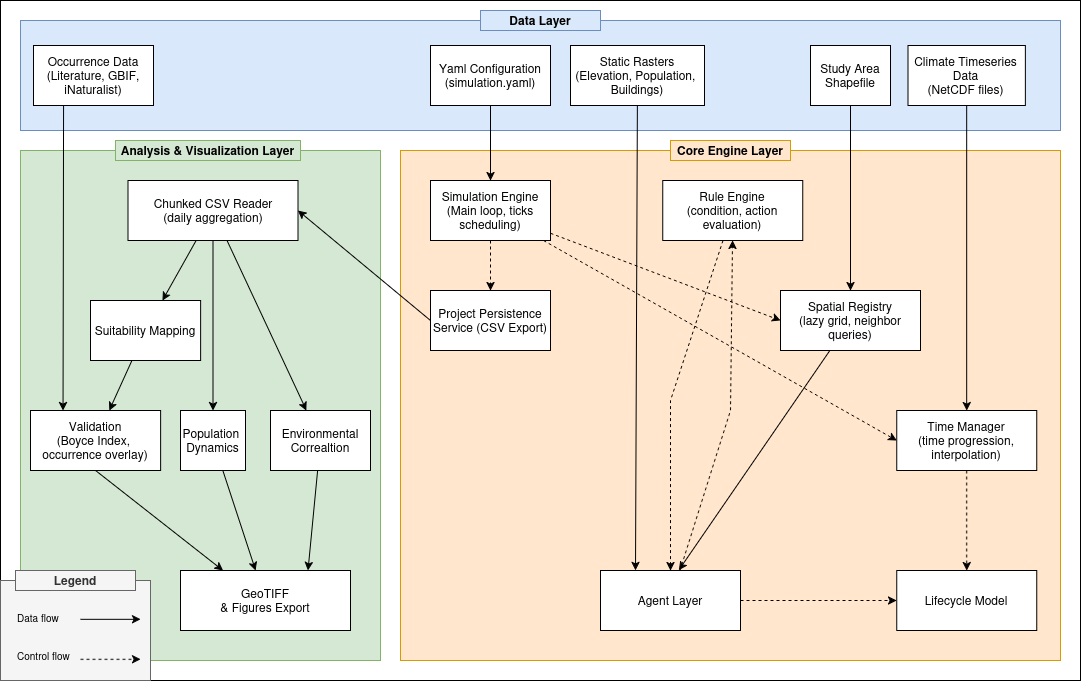
\includegraphics[width=\textwidth]{figs/phd_graphs-rmas.drawio.png}
\caption{High-level architecture of the simulation framework. The diagram is organised into three layers: 
\textit{Data Layer} (input data sources), \textit{Core Engine Layer} (simulation components), and \textit{Analysis 
\& Visualization Layer} (post-processing and validation). Solid arrows denote \textit{data flow} 
(e.g., configuration files, rasters, climate NetCDF, and simulation outputs). Dashed arrows denote 
\textit{control flow} (e.g., tick scheduling, spatial queries, rule evaluation, and lifecycle updates). The analysis 
layer reads CSV snapshots generated by the persistence service and produces daily summaries, suitability maps, 
validation metrics, and final figures.}
\label{fig:arch}
\end{figure}

\subsection{Core Components}
\label{sec:core_components}

\subsubsection{Agent layers}
Two agent types are implemented: \texttt{LivingAgent} (representing a mosquito) and \texttt{InertAgent} (representing a 
breeding site). Living agents track life stage (egg, larva, pupa, adult), age, energy, gravid status, and resting behaviour.
Their movement is modelled as a random walk with a step size derived from field observations of flight range \citep{1966.MA.FRL}. 
Inert agents maintain water volume, egg count, larval count, and carrying capacity; they update their capacity dynamically based on 
water level, mimicking density-dependent mortality observed in larval habitats \citep{2016.ST.OTI}. Agent layers are processed in 
parallel using a partition-based container (\texttt{AgentContainer}) and a rule engine that evaluates behavioural rules (e.g., 
feeding, oviposition, resting) in priority order \citep{2023.ST.ASR}.

\subsubsection{Raster layers and climate data}
Static raster layers (elevation, building density, population density) are loaded from GeoTIFF files using GeoTools and stored either 
in memory or memory-mapped for large grids. Climate time series (2-m temperature and total precipitation) are 
ingested from NetCDF files (ERA5-Land reanalysis) into interpolated raster layers that perform linear temporal interpolation between 
hourly steps \citep{2014.GC.AED, 2017.CL.IMS}.

\subsubsection{Lifecycle model}
\label{sec:lifecycle}

The lifecycle model follows the stage-structured discrete-time Metzler matrix framework from the work of \citet{2025.KM.WTR}. 
Four stages are tracked: eggs ($E$), larvae ($L$), pupae ($P$), and adult females ($A$). All rates are temperature-dependent 
and defined on a per-day basis. For a given daily rate $r$, the probability of transition or mortality over one tick of 
length $\Delta t$ (here $\Delta t = 0.01042$ days, corresponding to 15-minute ticks) is computed via the Poisson process:
\[
p = 1 - \exp(-r \Delta t).
\]
The daily projection matrix is:
\[
\mathbf{M}(T) = 
\begin{pmatrix}
(1 - d_E) S_E & 0 & 0 & F \cdot K \\
d_E S_E & (1 - d_L) S_L & 0 & 0 \\
0 & d_L S_L & (1 - d_P) S_P & 0 \\
0 & 0 & d_P S_P & 1 - \mu_A
\end{pmatrix},
\]
with stage abundances evolving as $[E, L, P, A]_{t+1}^\top = \mathbf{M}(T) [E, L, P, A]_t^\top$. The temperature-dependent 
functions are defined as follows.

\paragraph{Development rates} (units: $\mathrm{day}^{-1}$)
\begin{itemize}
  \item \textbf{Egg and pupa development} follow the Sharpe--Schoolfield type model:
  \[
  d_X(T) = \max \!\left(0, \rho e^{\rho k} e^{-\frac{k - T}{\Delta}} + \lambda \right),
  \]
  where $\rho$, $k$, $\Delta$, and $\lambda$ are species-specific parameters (see Table \ref{tab:lifecycle_params}).
  \item \textbf{Larva development} uses the Brière model:
  \[
  d_L(T) = \max \!\left(0, a T (T - T_{\min}) (T_{\max} - T)^{1/m} \right),
  \]
  with $a$, $T_{\min}$, $T_{\max}$, and $m$ as empirical coefficients.
\end{itemize}

\paragraph{Stage survival} (dimensionless)
Survival of eggs, larvae, and pupae is described by a Gaussian function:
\[
S_X(T) = \mathrm{amp}_X \cdot \exp \!\left( -\frac{1}{2} \left( \frac{T - \mu_X}{\sigma_X} \right)^2 \right).
\]

\paragraph{Adult mortality} ($\mathrm{day}^{-1}$)
Adult female mortality is temperature-dependent and modelled as an exponential quadratic:
\[
\mu_A(T) = \exp(b_1 + b_2 T + b_3 T^2),
\]
where $b_1, b_2, b_3$ are fitted coefficients.

\paragraph{Fecundity} (eggs per female per day)
Daily fecundity follows an asymmetric function:
\[
F(T) = \max \!\left(0, a e^{b T} - \exp \!\left( b T_{\max} - \left[ \frac{T_{\max} - T}{c} \right]^2 \right) \right),
\]
with parameters $a, b, T_{\max}$, and $c$.

\paragraph{Host carrying capacity}
Fecundity is multiplied by a dimensionless factor $K$ that accounts for human population density ($\mathrm{pop}$) and saturating effects:
\[
K = 1 + \ln(1 + \mathrm{pop}).
\]

\paragraph{Density-dependent larval mortality}
Each aquatic habitat (tank) has a carrying capacity $\mathrm{cap}$ that scales linearly with its water volume. If the number of 
larvae $L$ in a tank exceeds $\mathrm{cap}$, a proportion $(L - \mathrm{cap})/L$ of larvae is removed stochastically per tick, 
implementing a logistic-type density regulation.
\par
All temperature-response coefficients are stored in a YAML configuration file under the \texttt{species} key. The parameter 
names and corresponding YAML keys are listed in Table \ref{tab:lifecycle_params}.

\begin{table}[!htb]
\centering
\caption{Generic temperature-response parameters for the mosquito lifecycle model.}
\label{tab:lifecycle_params}
\small
\begin{tabular}{llll}
\toprule
Parameter & Meaning & Unit & YAML key \\ \midrule
\multicolumn{4}{l}{\textit{Egg and pupa development (Sharpe--Schoolfield)}} \\
$\rho$ & Development rate scale & $\mathrm{day}^{-1}$ & \texttt{egg\_dev\_rho}, \texttt{pupa\_dev\_rho} \\
$k$ & Optimal temperature & $^{\circ}\mathrm{C}$ & \texttt{egg\_dev\_k}, \texttt{pupa\_dev\_k} \\
$\Delta$ & Temperature sensitivity & $^{\circ}\mathrm{C}$ & \texttt{egg\_dev\_Delta}, \texttt{pupa\_dev\_Delta} \\
$\lambda$ & Baseline development offset & $\mathrm{day}^{-1}$ & \texttt{egg\_dev\_lambda}, \texttt{pupa\_dev\_lambda} \\ \addlinespace
\multicolumn{4}{l}{\textit{Larva development (Brière)}} \\
$a$ & Scaling factor & $\mathrm{day}^{-1} \, ^{\circ}\mathrm{C}^{-(1+1/m)}$ & \texttt{larva\_dev\_a} \\
$T_{\min}$ & Minimum temperature & $^{\circ}\mathrm{C}$ & \texttt{larva\_dev\_Tmin} \\
$T_{\max}$ & Maximum temperature & $^{\circ}\mathrm{C}$ & \texttt{larva\_dev\_Tmax} \\
$m$ & Shape exponent & --- & \texttt{larva\_dev\_m} \\ \addlinespace
\multicolumn{4}{l}{\textit{Stage survival (Gaussian)}} \\
$\mathrm{amp}_X$ & Maximum survival & --- & \texttt{<Stage>\_survival\_amp} \\
$\mu_X$ & Optimum temperature & $^{\circ}\mathrm{C}$ & \texttt{<Stage>\_survival\_mean} \\
$\sigma_X$ & Temperature tolerance width & $^{\circ}\mathrm{C}$ & \texttt{<Stage>\_survival\_sigma}\\ \addlinespace
\multicolumn{4}{l}{\textit{Adult mortality (exponential quadratic)}} \\
$b_1$ & Intercept & --- & \texttt{adult\_mort\_b1} \\
$b_2$ & Linear coefficient & $^{\circ}\mathrm{C}^{-1}$ & \texttt{adult\_mort\_b2} \\
$b_3$ & Quadratic coefficient & $^{\circ}\mathrm{C}^{-2}$ & \texttt{adult\_mort\_b3} \\ \addlinespace
\multicolumn{4}{l}{\textit{Fecundity}} \\
$a$ & Maximum fecundity scale & eggs/fem/day & \texttt{fecundity\_rmax} \\
$b$ & Exponential coefficient & $^{\circ}\mathrm{C}^{-1}$ & \texttt{fecundity\_c} \\
$T_{\max}$ & Temp. of max fecundity & $^{\circ}\mathrm{C}$ & \texttt{fecundity\_Topt} \\
$c$ & Quadratic decay parameter & $^{\circ}\mathrm{C}^{-2}$ & \texttt{fecundity\_c} \\ 
\bottomrule
\end{tabular}
\end{table}

\subsubsection{Rule engine and spatial registry}
Behavioural rules (e.g., "\texttt{feed}", "\texttt{lay\_eggs}", "\texttt{rest\_in\_building}") are defined in a YAML configuration 
file and evaluated using a JavaScript engine (GraalVM \citep{2023.VT.CPA}). The spatial registry implements a lazy grid with a configurable cell size 
(default $0.001^\circ \approx 110$ m). Neighbour queries are performed by checking cells within a Chebyshev distance 
$\lceil \text{radius}/\text{cellSize}\rceil$; results are cached for one second per cell to reduce computational cost.

\subsubsection{Simulation Configuration}
\par
All simulation parameters are defined in a single YAML file (\texttt{simulation.yaml}). The file specifies:  
\par
\begin{itemize}
  \item \textbf{Time settings}: start date, total number of ticks, tick duration (15-minutes).  
  \item \textbf{File paths}: study area shapefile, elevation, building density, population rasters, and the climate NetCDF.  
  \item \textbf{Species parameters}: coefficients for development, survival, fecundity, and adult mortality.  
  \item \textbf{Tokens}: mapping between environment variable names (e.g., "temperature") and raster layers.  
  \item \textbf{Agent layers and rules}: each layer contains a list of rules with a condition, an action, and a priority.  
  \item \textbf{Seeding}: number of breeding sites and mosquitoes, habitat grid resolution, and whether to seed uniformly or 
  using a weighted habitat suitability map.  
  \item \textbf{Project defaults}: agent search radius, step size, maximum age.
\end{itemize}
\par
At startup, the simulator loads the configuration, initialises the time manager, loads rasters and climate data, 
creates the spatial registry, builds agent layers, seeds the initial population, and starts the simulation engine.

\subsubsection{Result Analysis}
\label{sec:analysis}
\par
Simulation outputs are exported as CSV snapshots every 100 ticks. Each snapshot contains per-agent records 
with tick count, agent ID, layer, type, coordinates, alive flag, age, stage, energy, gravid status, and for inert agents, egg/larval 
counts and water volume. Environmental values (temperature, precipitation, etc) are attached to each agent's row via bilinear interpolation 
from the current climate frame.
\par
The analysis, visulization and validation of the resutls are realized through a jupyter notebook (Python) which performs the following steps:
\par
\begin{enumerate}
  \item \textbf{Daily aggregation}: The CSV is read in chunks (100 000 rows) to compute daily adult, larva, and pupa counts, as well 
  as breading sites statistics (mean water volume, total eggs/larvae), using the tick-to-day conversion ($96$ ticks per day by default).  
  \item \textbf{Population dynamics}: Stage counts are plotted, and stage durations are estimated from cross-correlation of smoothed 
  population peaks. Theoretical durations are computed from species parameters at the mean observed temperature.  
  \item \textbf{Environmental correlation}: Pearson correlation between daily adult counts and mean temperature / precipitation is calculated.  
  \item \textbf{Suitability mapping}: A kernel density estimate (KDE) of adult points (bandwidth $0.002^{\circ} \approx 220 m$) is generated and exported 
  as a GeoTIFF. A breeding site potential raster is created by rasterising the sum of eggs and larvae in water tanks on the last tick.  
  \item \textbf{Validation}: The continuous Boyce index \citep{2006.HA.ETA} and the proportion of occurrence points falling into the top 20\% 
  of the suitability surface are computed using independently collected occurrence data (from GBIF, iNaturalist, literature, clipped to 
  the study area).  
  \item \textbf{Export}: Daily summaries and a sample of raw data are saved for further analysis.
\end{enumerate}
\par
All figures and rasters are stored in a user-defined output directory.

\subsection{Case Study Design}
\label{sec:case_study}
\subsubsection{Vector and Study Site}
\par
The case study is set in Ethiopia, focusing on two contrasting regions: Somali and Oromia. 
Both areas have experienced recent incursions of the Asian malaria vector \textit{Anopheles stephensi} and are 
considered high-risk zones for urban and peri-urban malaria transmission \citep{2020.MB.GDO, 2021.MB.AUO, 2023.DH.FRO}.
\par
Somali (\ang{6.6612} N, \ang{43.7908} E) is is characterized by a hot, semi-arid climate and a known 
history of \textit{An. stephensi} establishment, first reported in 2018 \citep{2020.MB.GDO}. The Oromia (\ang{7.5460} N, \ang{40.6347} E) 
study area comprises several districts that span an altitudinal gradient from \SIrange{1500}{2500}{\meter}, representing a mix of 
agricultural, peri-urban, and highland ecosystems where the vector has been detected since 2019 \citep{2021.MB.AUO, 2024.TA.SDA}. 
These sites were selected because they provide a natural experiment to evaluate the simulator's 
ability to capture spatial heterogeneity in vector abundance driven by temperature, urbanisation, and host availability 
\citep{2025.TD.BOA, 2024.GZ.ROC}.

\subsubsection{Vector Biology}
\label{sec:stephensi_lifecycle}

\textit{Anopheles stephensi} is a highly adaptive urban malaria vector native to South Asia and the Middle East, now established 
in the Horn of Africa \citep{2024.RT.IAS}. Its life cycle is tightly coupled to temperature, and its larvae exploit a wide range 
of artificial containers, especially overhead water tanks and construction pits \citep{2016.ST.OTI}. 

The temperature-dependent functions described in Section \ref{sec:lifecycle} were parameterised for \textit{An. stephensi}. 
The coefficients (Table \ref{tab:stephensi_params}) were obtained by fitting laboratory and field data from 
\citet{2023.NT.EOT}, \citet{2022.OC.TIT}, and \citet{1980.WK.HLT} using a Python notebook ( see 
\texttt{species\_parameters\_extraction.ipynb} in the code linked to this work -- Section \ref{sec:data_availability}). 
All fitted parameters are stored in the file \texttt{species\_parameters.yaml}.

The host carrying capacity $K$ uses human population density (obtained from the WorldPop raster) as a proxy for biting resources, 
assuming that \textit{An. stephensi} is highly anthropophilic in urban settings \citep{2024.TA.SDA, 2022.AH.TPI}. Density-dependent 
larval mortality follows the tank capacity model of \citet{2016.ST.OTI}, where capacity is linearly scaled with water volume 
(maximum 500 larvae at \SI{100}{\percent} water volume).

\begin{table}[!htb]
\centering
\small
\caption{Species-specific parameters for \textit{Anopheles stephensi} used in the case study.}
\label{tab:stephensi_params}
\begin{tabular}{@{}llcl@{}}
\toprule
Parameter & Meaning & Value / coefficients & Source \\ \midrule
\multicolumn{4}{l}{\textit{Development rates}} \\ \addlinespace
$d_E$ & Egg dev. ($\mathrm{day}^{-1}$) & $\rho = 0.0050, k = 39.208, \Delta = 2.000, \lambda = -0.855$ & \cite{1980.WK.HLT} \\
$d_L$ & Larva dev. ($\mathrm{day}^{-1}$) & $a = 2.71 \times 10^{-5}, T_0 = 5.12, T_m = 45.00, m = 1.66$ & \cite{2022.OC.TIT} \\
$d_P$ & Pupa dev. ($\mathrm{day}^{-1}$) & $\rho = 0.0051, k = 39.940, \Delta = 2.000, \lambda = -0.908$ & \cite{2023.NT.EOT} \\ \midrule
\multicolumn{4}{l}{\textit{Mortality rates [$\exp(b_1+b_2T+b_3T^2)$]}} \\ \addlinespace
$\mu_E$ & Egg mort. ($\mathrm{day}^{-1}$) & $b_1 = 3.5729, b_2 = -0.3235, b_3 = 0.00494$ & \cite{1980.WK.HLT} \\
$\mu_L$ & Larva mort. ($\mathrm{day}^{-1}$) & $b_1 = 2.0000, b_2 = -0.7395, b_3 = 0.01749$ & \cite{2022.OC.TIT} \\
$\mu_P$ & Pupa mort. ($\mathrm{day}^{-1}$) & $b_1 = 5.8826, b_2 = -0.5785, b_3 = 0.00946$ & \cite{2023.NT.EOT} \\
$\mu_A$ & Adult mort. ($\mathrm{day}^{-1}$) & $b_1 = -1.4775, b_2 = -0.1377, b_3 = 0.00391$ &  \\
& Constant adult mort. & $\mu_A^{\mathrm{const}} = 0.1198$ & - \\ \midrule
\multicolumn{4}{l}{\textit{Fecundity and sex ratio}} \\ \addlinespace
$F$ & Fecundity & $r_{\max}=1.602, T_{\mathrm{opt}}=30.634, c=-0.00527$ & \cite{2022.OC.TIT} \\
& Sex ratio & 0.5 & Assumed \\ \midrule
\multicolumn{4}{l}{\textit{Carrying capacity}} \\ \addlinespace
$K$ & Host scaling factor & $1 + \ln(1+\mathrm{popdens})$ & WorldPop \citet{2020.RC.MGP} \\ \bottomrule
\end{tabular}
\end{table}


\subsubsection{Data Sources}
\label{sec:data_sources}

The simulation integrates five categories of data:

\begin{itemize}
    \item \textbf{Static environmental rasters} -- Elevation (SRTM, \SI{30}{\meter}), building density (Global 
	Human Settlement Layer), and human population density (WorldPop, 2020) were resampled to a common \ang{0.001} 
	(\SI{\sim 110}{\meter}) grid over the study area.
    
    \item \textbf{Climate time series} -- Hourly \SI{2}{\meter} temperature and total precipitation for 2020 were 
	obtained from the ERA5-Land reanalysis (Copernicus Climate Change Service) and stored as NetCDF files.
    
    \item \textbf{Vector occurrence data} -- Presence points for \textit{An. stephensi} in Ethiopia were compiled from 
	the Vector Atlas database \citep{2025.VE.VAP}, GBIF \citep{2011.AN.BIG}, and recent entomological surveys 
	\citep{2020.MB.GDO, 2021.MB.AUO, 2023.DH.FRO}. Only records with precise coordinates and collection dates 
	in 2018--2022 were retained.
    
    \item \textbf{Bionomic and life-history data} -- Parameter values (Table \ref{tab:stephensi_params}) were extracted 
	from peer-reviewed literature \citep{2022.OC.TIT, 2023.JJ.BBA, 2025.CG.EOT} and supplemented with expert knowledge.
    
\end{itemize}

All data were harmonised to the WGS-84 geographic coordinate system (EPSG:4326) and stored in a structured file hierarchy.

\subsubsection{Simulation Assupmtions, Rules and Configuration}
\label{sec:sim_assumptions}

The simulation makes the following key assumptions:
\begin{enumerate}  
    \item \textbf{Temperature is the primary abiotic driver} -- All development, survival, and reproduction rates respond 
	only to ambient temperature; effects of relative humidity, rainfall, and other variables are omitted or implicitly 
	captured through breeding site water dynamics.  
    
    \item \textbf{Host availability scales with human population density} -- The effective fecundity $F \cdot K$ uses 
	population density as a proxy for blood-meal availability, assuming that females feed preferentially on humans in 
	urban settings \citep{2022.AH.TPI}.  
    
    \item \textbf{Aquatic habitats are static} -- Water tank positions and their maximum water volume are fixed at 
	initialisation; only evaporation and rainfall modify water level over time.  
    
    \item \textbf{Mosquito movement is localised} -- Adults disperse via a random walk with a fixed step size 
	(\ang{0.00005} $\approx$ \SI{5.5}{\meter} per tick) and a search radius of \ang{0.005} (\SI{\sim 550}{\meter}), 
	reflecting limited flight range \citep{1966.MA.FRL}.  
    
    \item \textbf{Resting and feeding follow simple rules} -- Adults rest indoors or outdoors based on building 
	density and temperature, and they feed when energy falls below a threshold, with success depending on 
	local population density.
\end{enumerate}

The behavioural rules (Table \ref{tab:rules}) are encoded in the YAML configuration file (\texttt{simulation.yaml}) and 
evaluated in priority order at each tick. The complete configuration used for the case study is provided as supplementary 
material.

\begin{table}[!htb]
\centering
\caption{Behavioural rules for \textit{An. stephensi} adults.}
\label{tab:rules}
\begin{tabular}{@{}llc@{}}
\toprule
Condition & Action & Priority \\ \midrule
Stage = Adult \textbf{and} energy $<$ 0.6 \textbf{and} not resting & \texttt{feed} & 8 \\
Stage = Adult \textbf{and} energy $>$ 0.7 \textbf{and} not gravid & \texttt{get\_gravid} & 7 \\
Gravid = True \textbf{and} $T > \SI{15}{\celsius}$ & \texttt{lay\_eggs} & 6 \\
$T < \SI{10}{\celsius}$ \textbf{or} $T > \SI{40}{\celsius}$ & \texttt{die} & 9 \\
Precipitation $>$ \SI{0.008}{\meter} \textbf{and} build. dens. $>$ 0.1 \textbf{and} not resting & \texttt{rest\_in\_building} & 5 \\
Stage = Adult \textbf{and} not resting & \texttt{move\_random} & 3 \\
Otherwise & \texttt{rest} & 2 \\ \bottomrule
\end{tabular}
\end{table}

The simulation was run for 180 days (six months, tick = \SI{15}{\minute}, \num{17280} ticks) with a burn-in of 5 days 
to allow transients to decay. Output snapshots were exported every 100 ticks and analysed using the Python notebook described in 
Section \ref{sec:analysis}.

\subsubsection{Experimental Setup}
All simulations were executed on a laptop equipped with an Intel Core i5-6300U processor (2 physical cores, 4 threads, base frequency 
\SI{2.40}{\giga\hertz}, max turbo \SI{3.00}{\giga\hertz}) and \SI{8}{\giga\byte} of RAM. The operating system was Linux (x86\_64), 
and the Java Virtual Machine (JVM) was configured with a maximum heap size of \SI{1950}{\mega\byte} (approximately \SI{80}{\percent} of physical memory). 
The simulation engine used a thread pool with three worker threads (one less than the total number of logical threads) to avoid 
oversubscription. The spatial registry implemented a lazy grid with a cell size of \SI{0.001}{\degree} ($\approx$\SI{110}{\meter}). 
Each simulation ran for 180 simulated days (\num{17280} ticks of \SI{15}{\minute}). Output snapshots were exported every 100 ticks. 
The analysis notebook (Python 3.10) was executed on the same hardware.


\section{Results}
\label{sec:results}

The simulation was executed for a duration of six months (180 days, comprising \num{17280} ticks of \qty{15}{\minute} each) over 
the contrasting study areas of Somali and Oromia in Ethiopia. The model utilised the temperature-dependent lifecycle parameters 
specifically fitted for \textit{Anopheles stephensi}. Output snapshots were processed to evaluate population stability, environmental 
response, and spatial suitability.

\subsection{Population Dynamics and Lifecycle Validation}

In the Oromia region, the mosquito population reached a near-steady state after approximately 10 days of simulation, with adult abundance 
stabilising at approximately \num{85000} individuals, while larval and pupal counts fluctuated around \num{36000} and \num{21600}, 
respectively (Figure~\ref{fig:population_dynamics}). Analysis of the six-month time series revealed that the daily adult count maintained 
a weak positive correlation with temperature (Pearson's $r = 0.119$, $p = 0.12$) and a stronger positive correlation with 
precipitation ($r = 0.618$, $p = 1.56\times10^{-19}$).

In the Somali region, the adult count started at approximately \num{131000} and showed a slow but consistent increase, with larvae 
and pupae averaging \num{54700} and \num{32700}, respectively. Temperature remained nearly constant (\qty{26.3 \pm 0.1}{\celsius}) 
throughout the simulation, leading to an undefined correlation coefficient. Precipitation exhibited a moderate negative correlation 
with adult abundance ($r = -0.477$, $p = 3.8\times10^{-11}$). These results indicate that under the simulated conditions, intrinsic 
density-dependent regulation and the availability of stable aquatic habitats dominated over short-term climatic fluctuations in both regions.

Theoretical stage durations were calculated based on the mean observed temperatures: at \qty{21.5}{\celsius} (Oromia) the larval and 
pupal stages lasted \qty{15.7}{\day} and \qty{4.8}{\day}, respectively; at \qty{26.3}{\celsius} (Somali) the corresponding durations 
were \qty{11.4}{\day} and \qty{4.3}{\day}. The dominant eigenvalue ($\lambda_{\max}$) of the Metzler projection matrix, averaged over 
the full simulation period, was \num{1.077} for Oromia and \num{1.135} for Somali. These values indicate a slowly growing population 
approaching equilibrium, consistent with the established status of \textit{An. stephensi} in urban Ethiopia \citep{2021.MB.AUO}. 
Figure~\ref{fig:growth} illustrates the observed daily adult growth factor alongside the predicted $\lambda_{\max}$.

\begin{figure}[!htb]
    \centering
    \begin{subfigure}[b]{0.48\textwidth}
        \centering
        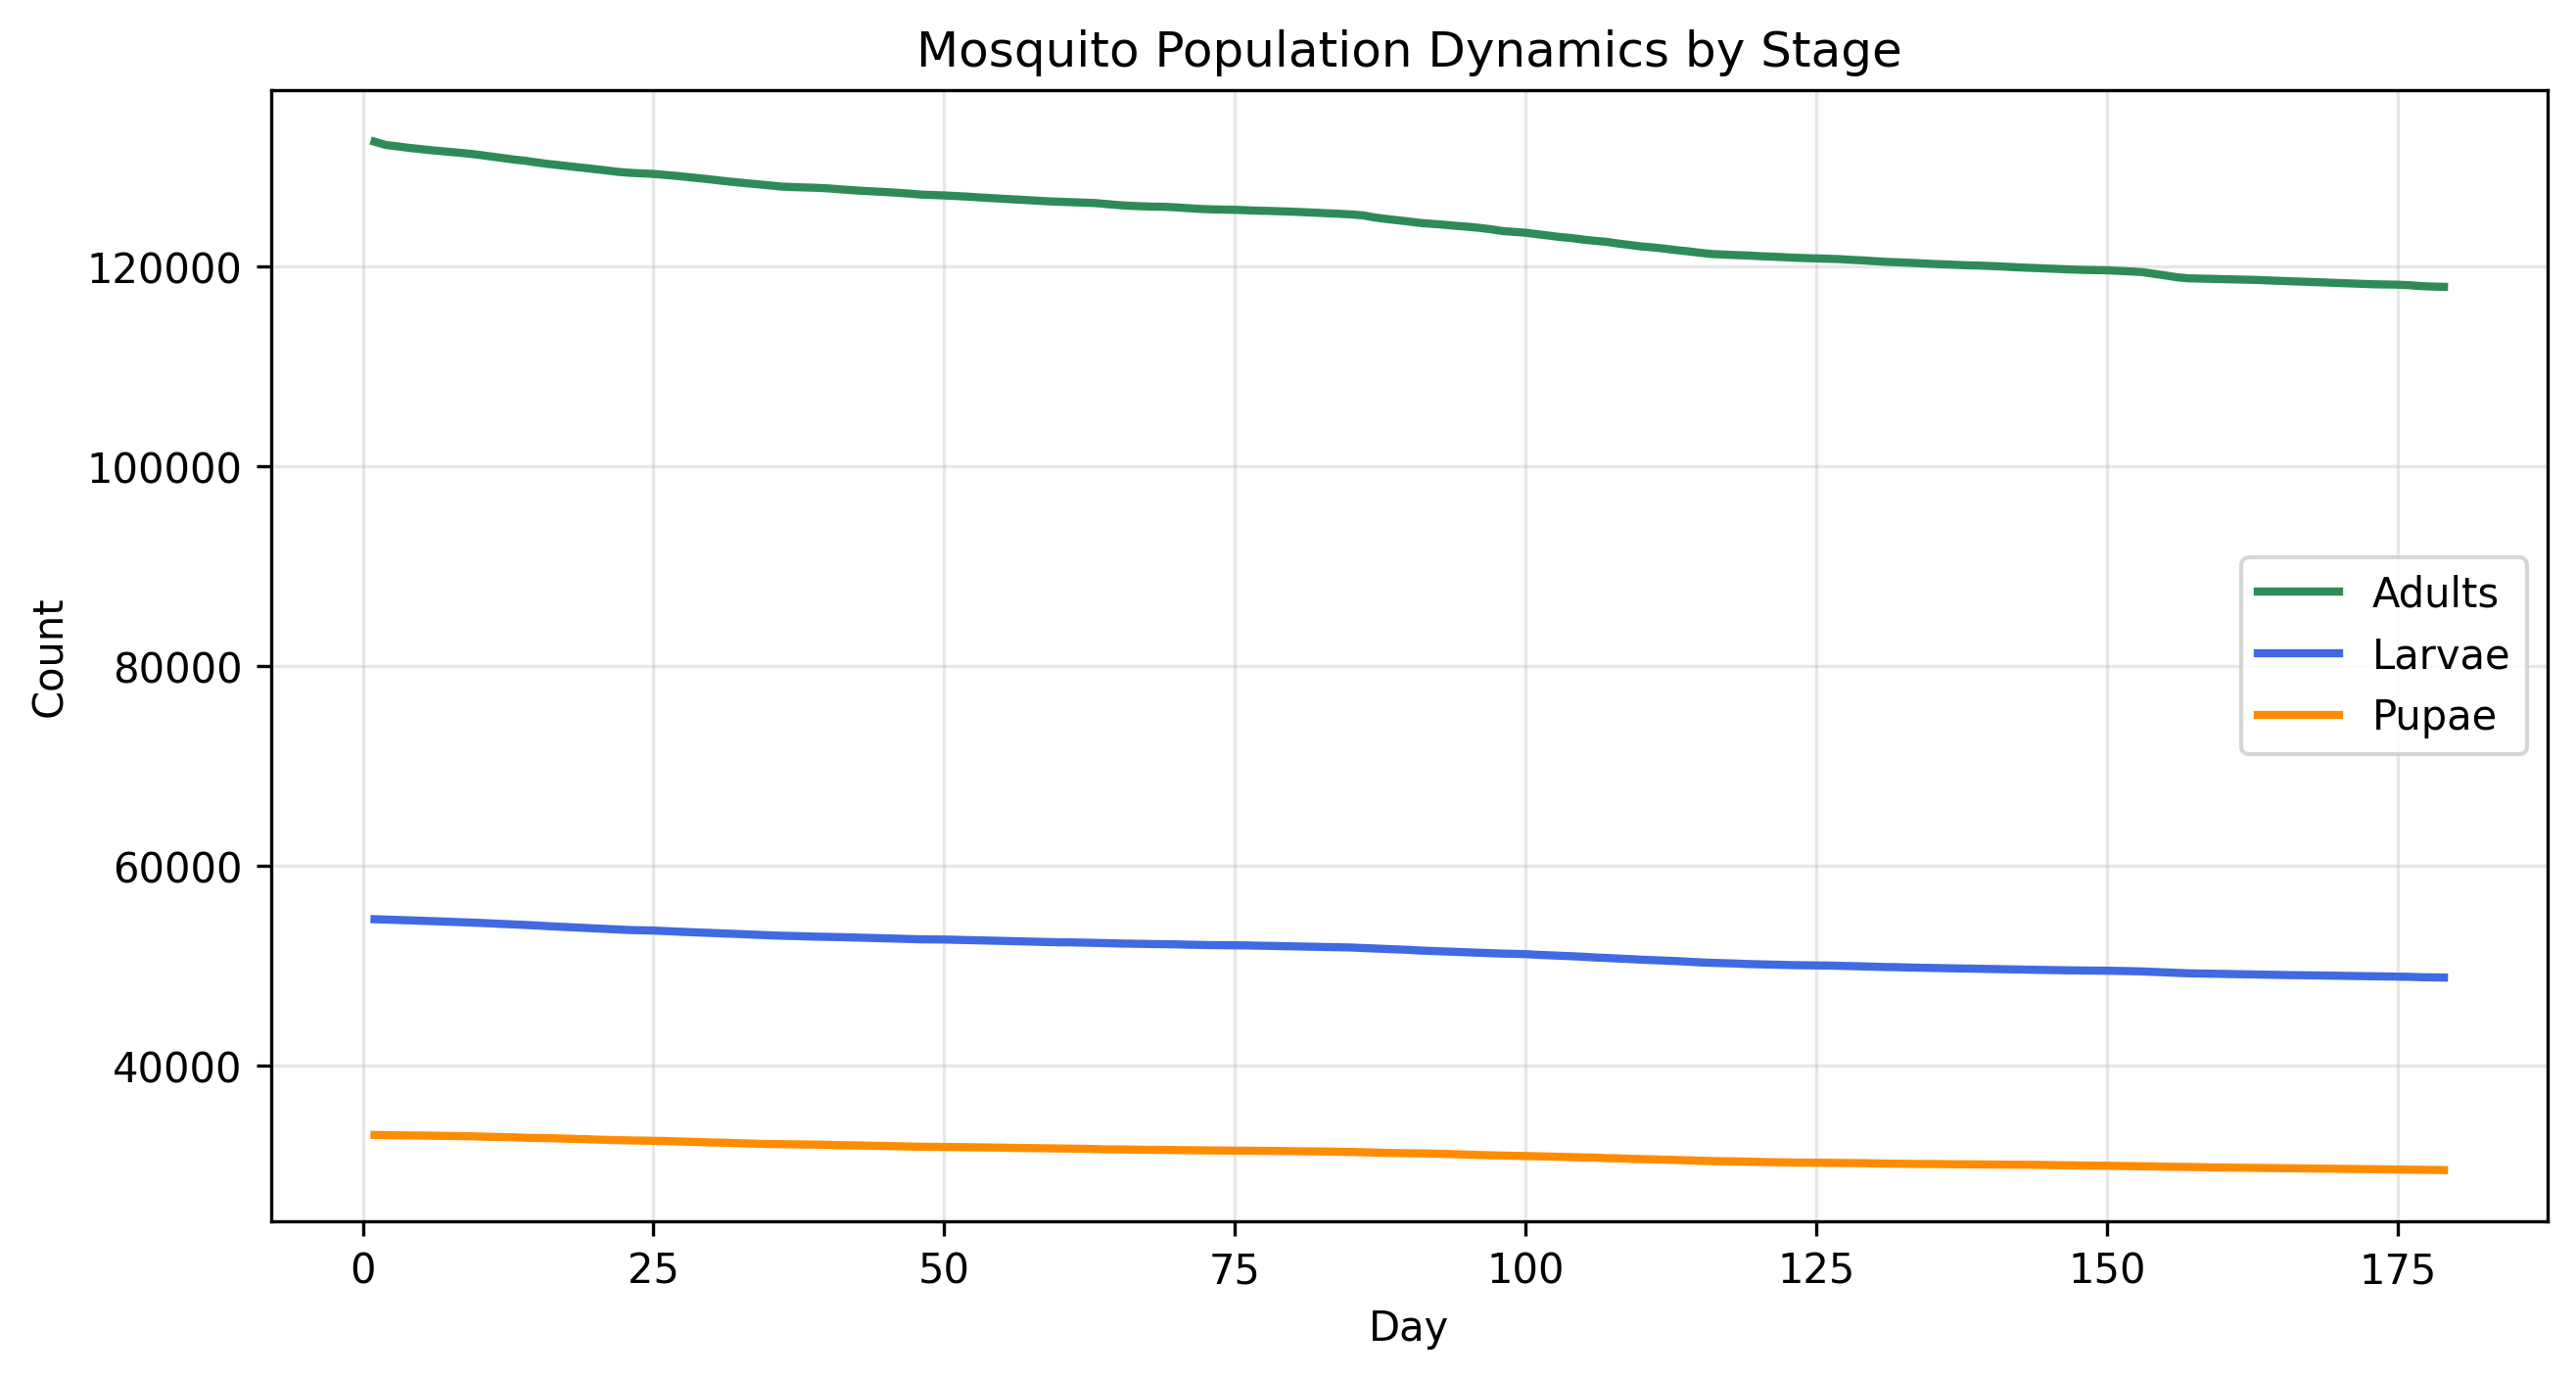
\includegraphics[width=\textwidth]{figs/somali/mosquito_dynamics.png}
        \caption{Somali}
    \end{subfigure}
    \hfill
    \begin{subfigure}[b]{0.48\textwidth}
        \centering
        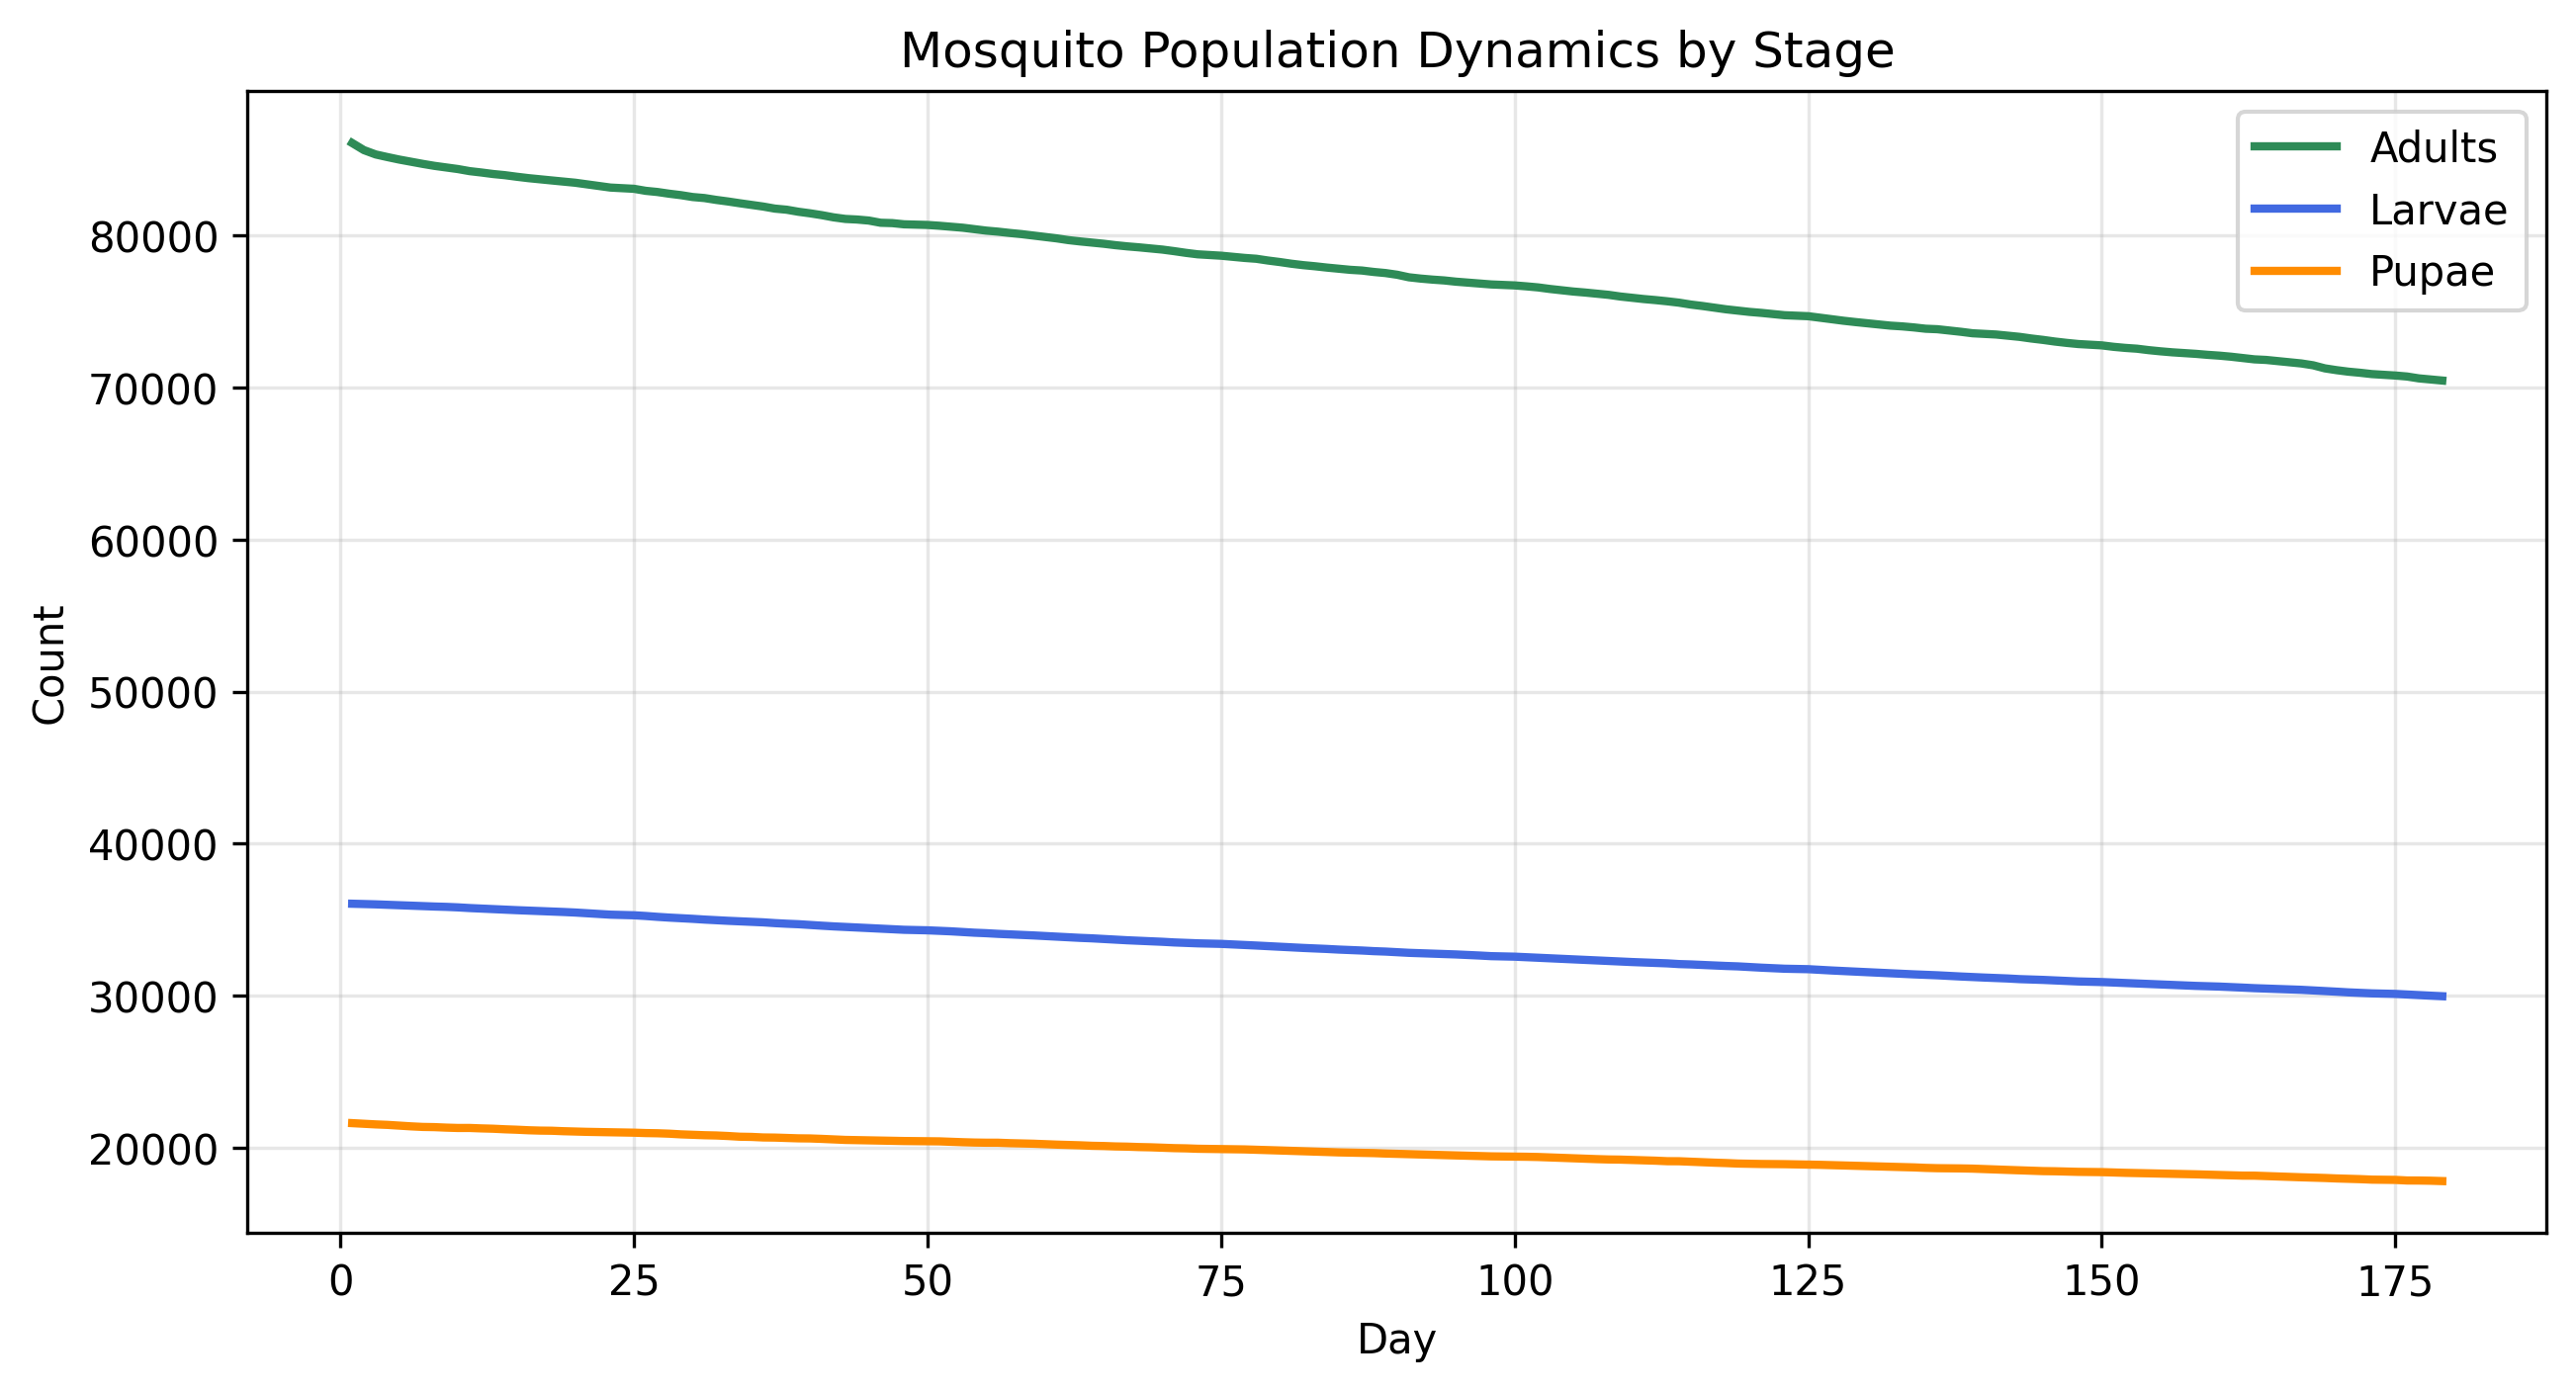
\includegraphics[width=\textwidth]{figs/oromia/mosquito_dynamics.png}
        \caption{Oromia}
    \end{subfigure}
    \caption{Daily counts of adult, larval, and pupal \textit{An. stephensi} over the six-month simulation. Population levels 
    stabilised after an initial burn-in period of about 10 days.}
    \label{fig:population_dynamics}
\end{figure}

\begin{figure}[!htb]
    \centering
    \begin{subfigure}[b]{0.48\textwidth}
        \centering
        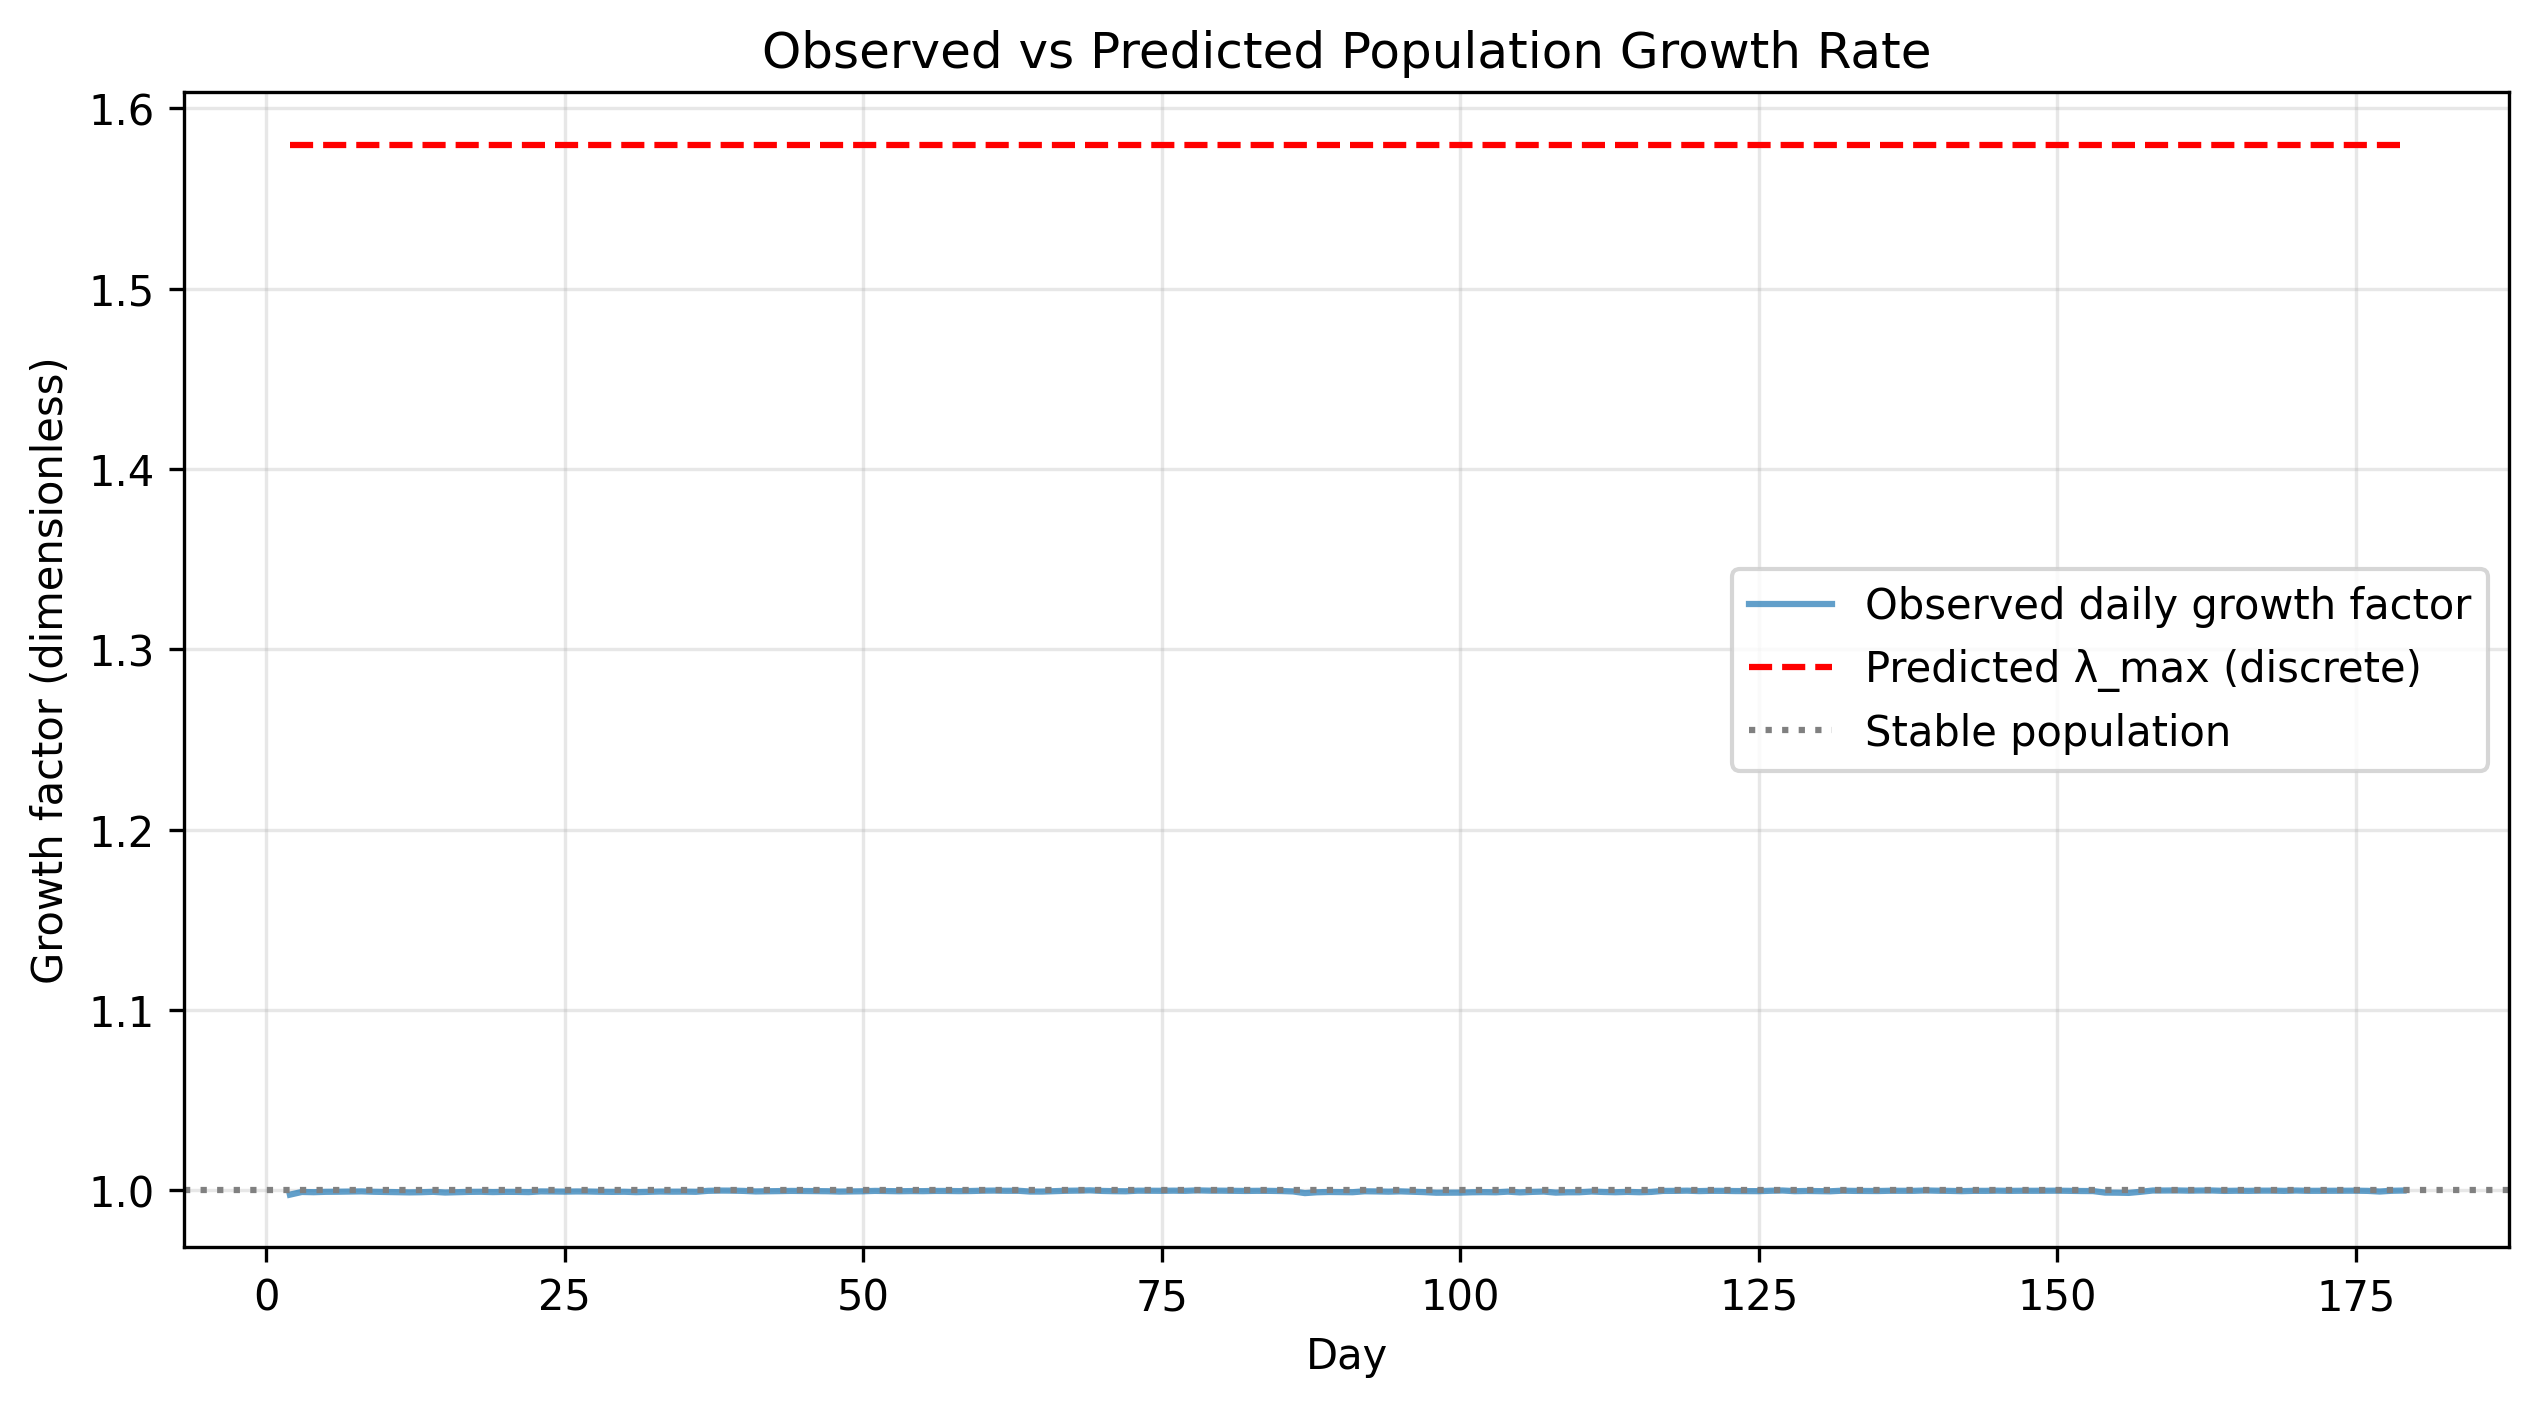
\includegraphics[width=\textwidth]{figs/somali/growth_validation.png}
        \caption{Somali}
    \end{subfigure}
    \hfill
    \begin{subfigure}[b]{0.48\textwidth}
        \centering
        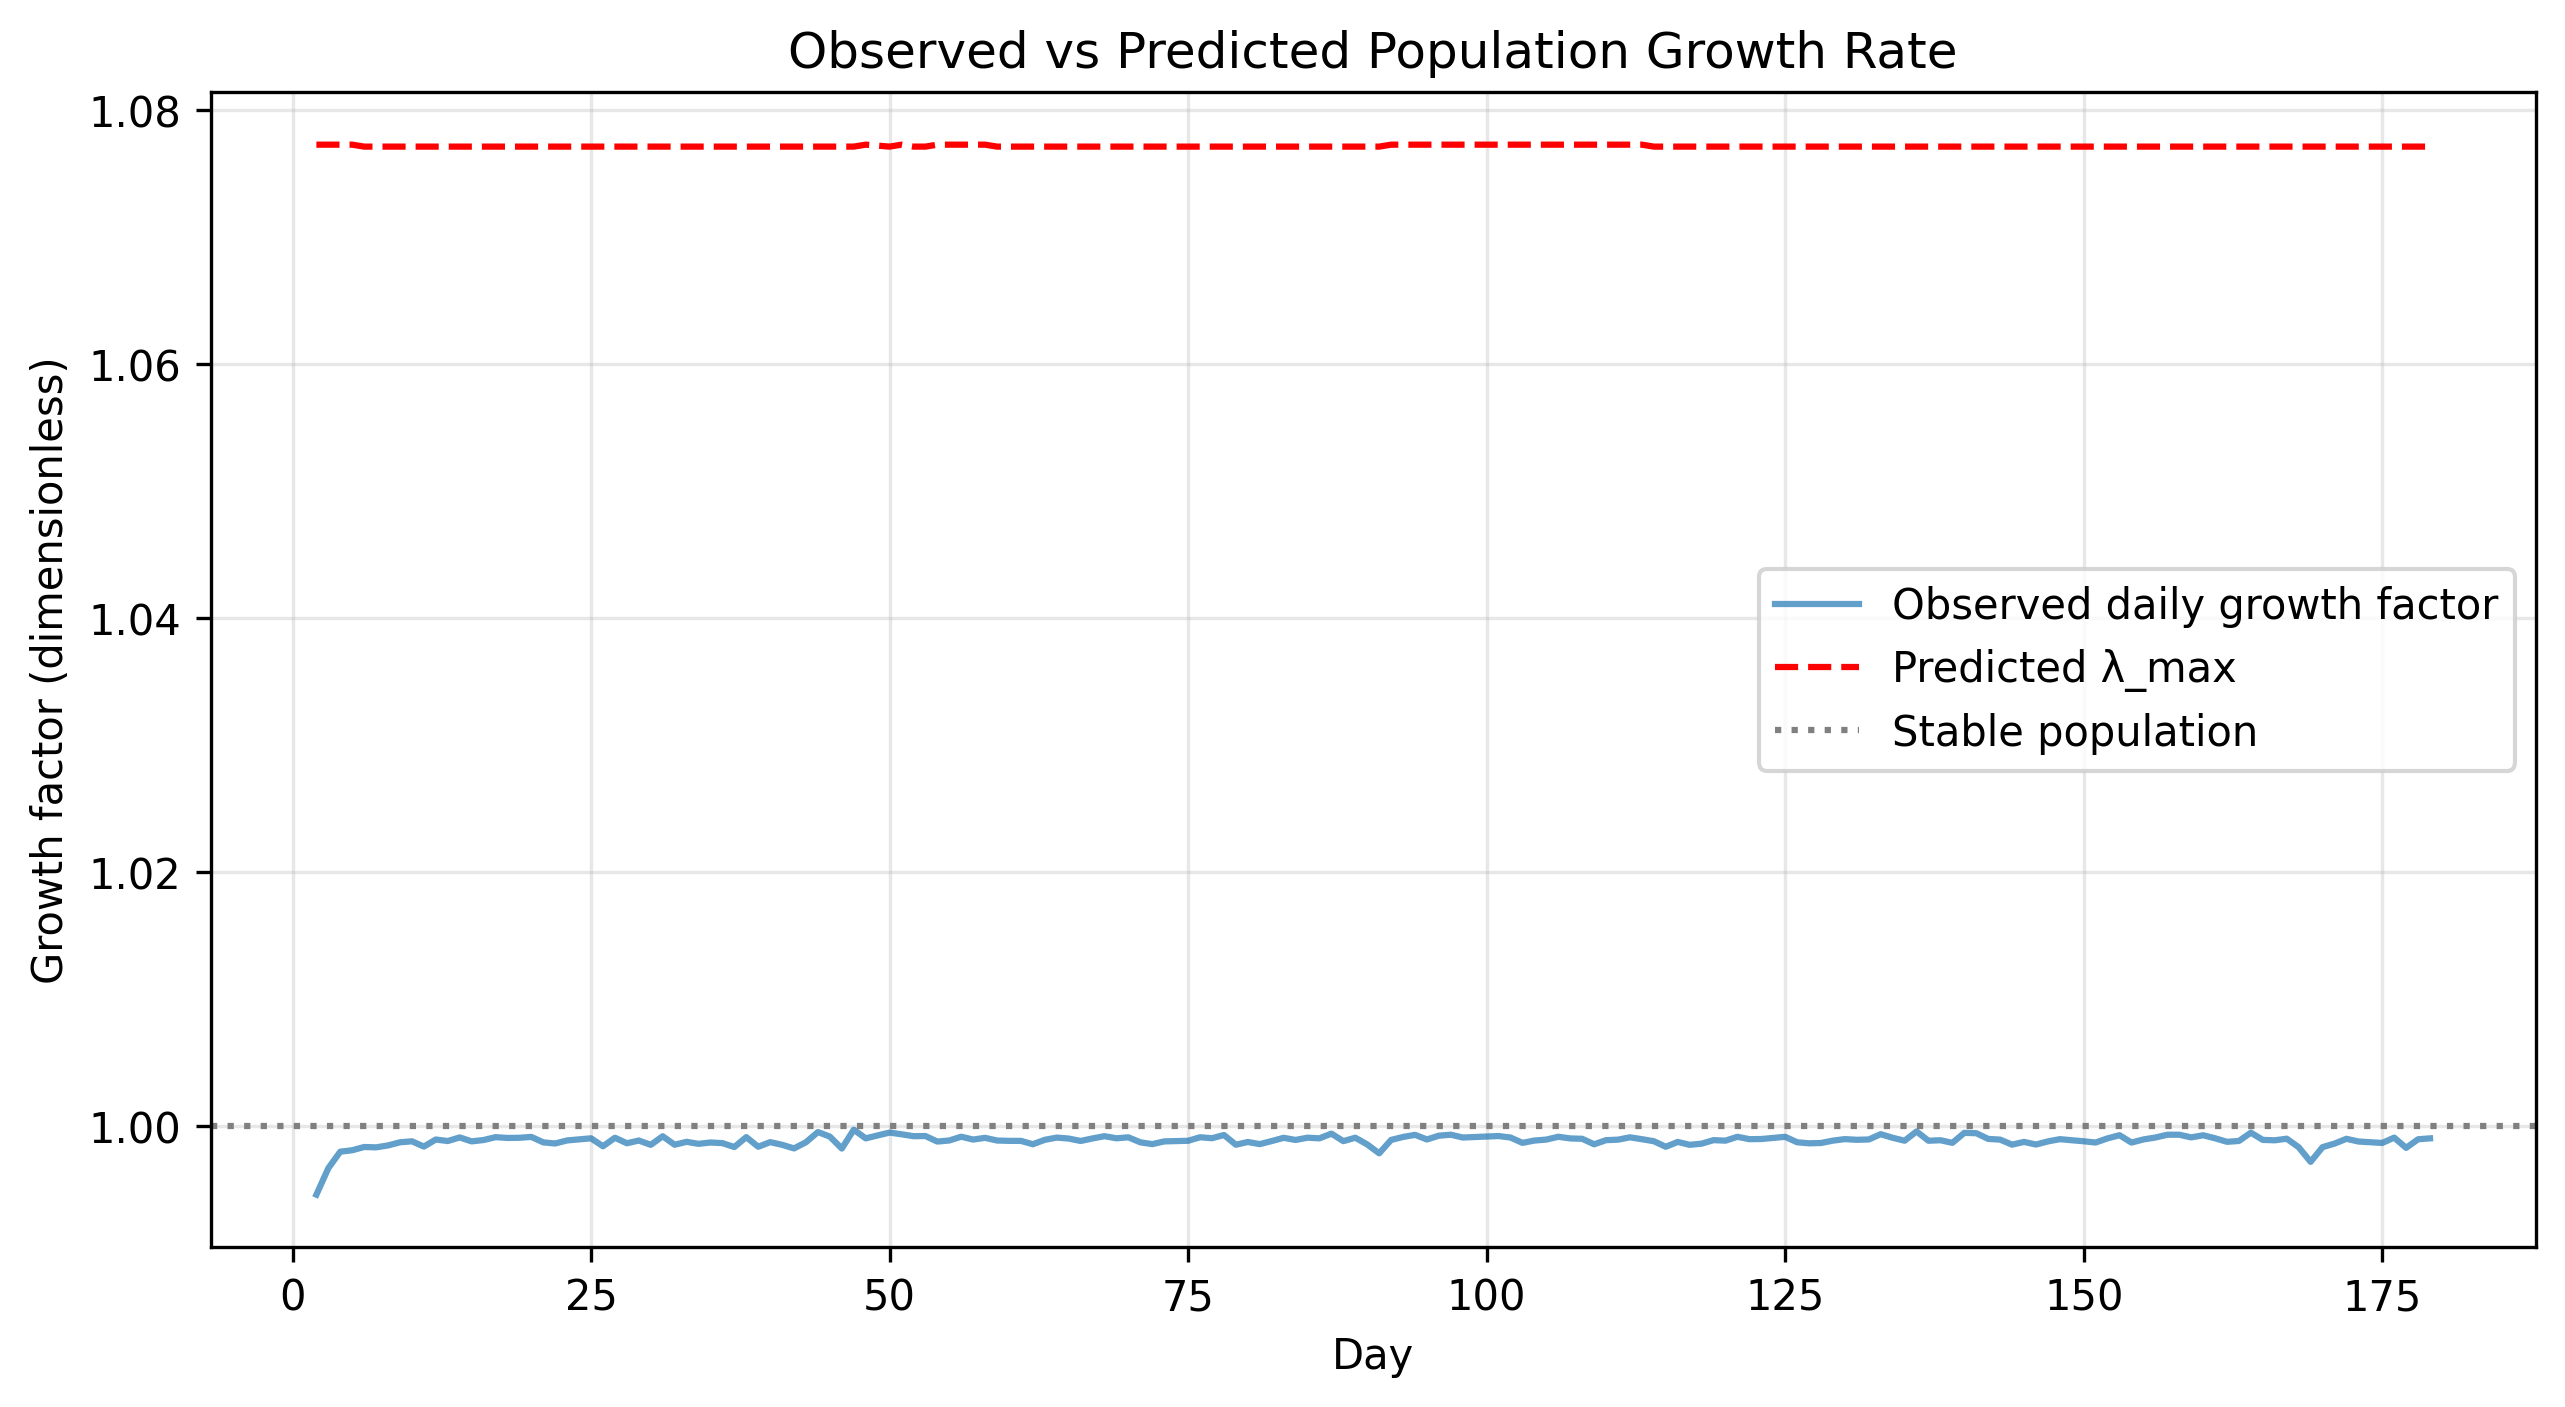
\includegraphics[width=\textwidth]{figs/oromia/growth_validation.png}
        \caption{Oromia}
    \end{subfigure}
    \caption{Observed daily adult growth factor versus predicted $\lambda_{\max}$ (red dashed line). The average predicted 
    growth factor closely matches the observed stability in both regions.}
    \label{fig:growth}
\end{figure}

\subsection{Water Tank Statistics}

The Oromia simulation included 474 water tanks, while the Somali simulation included 42 tanks. In both regions, mean water volume 
remained highly stable ($\qty{84.6 \pm 0.1}{\percent}$ for Oromia, $\qty{83.7 \pm 0.0}{\percent}$ for Somali), as evaporation 
losses were balanced by periodic precipitation events (Figure~\ref{fig:tank_stats}). The reciprocal trend between egg and larval 
counts per tank confirmed active hatching and stage transition within these permanent aquatic habitats.

\begin{figure}[!htb]
    \centering
    \begin{subfigure}[b]{0.48\textwidth}
        \centering
        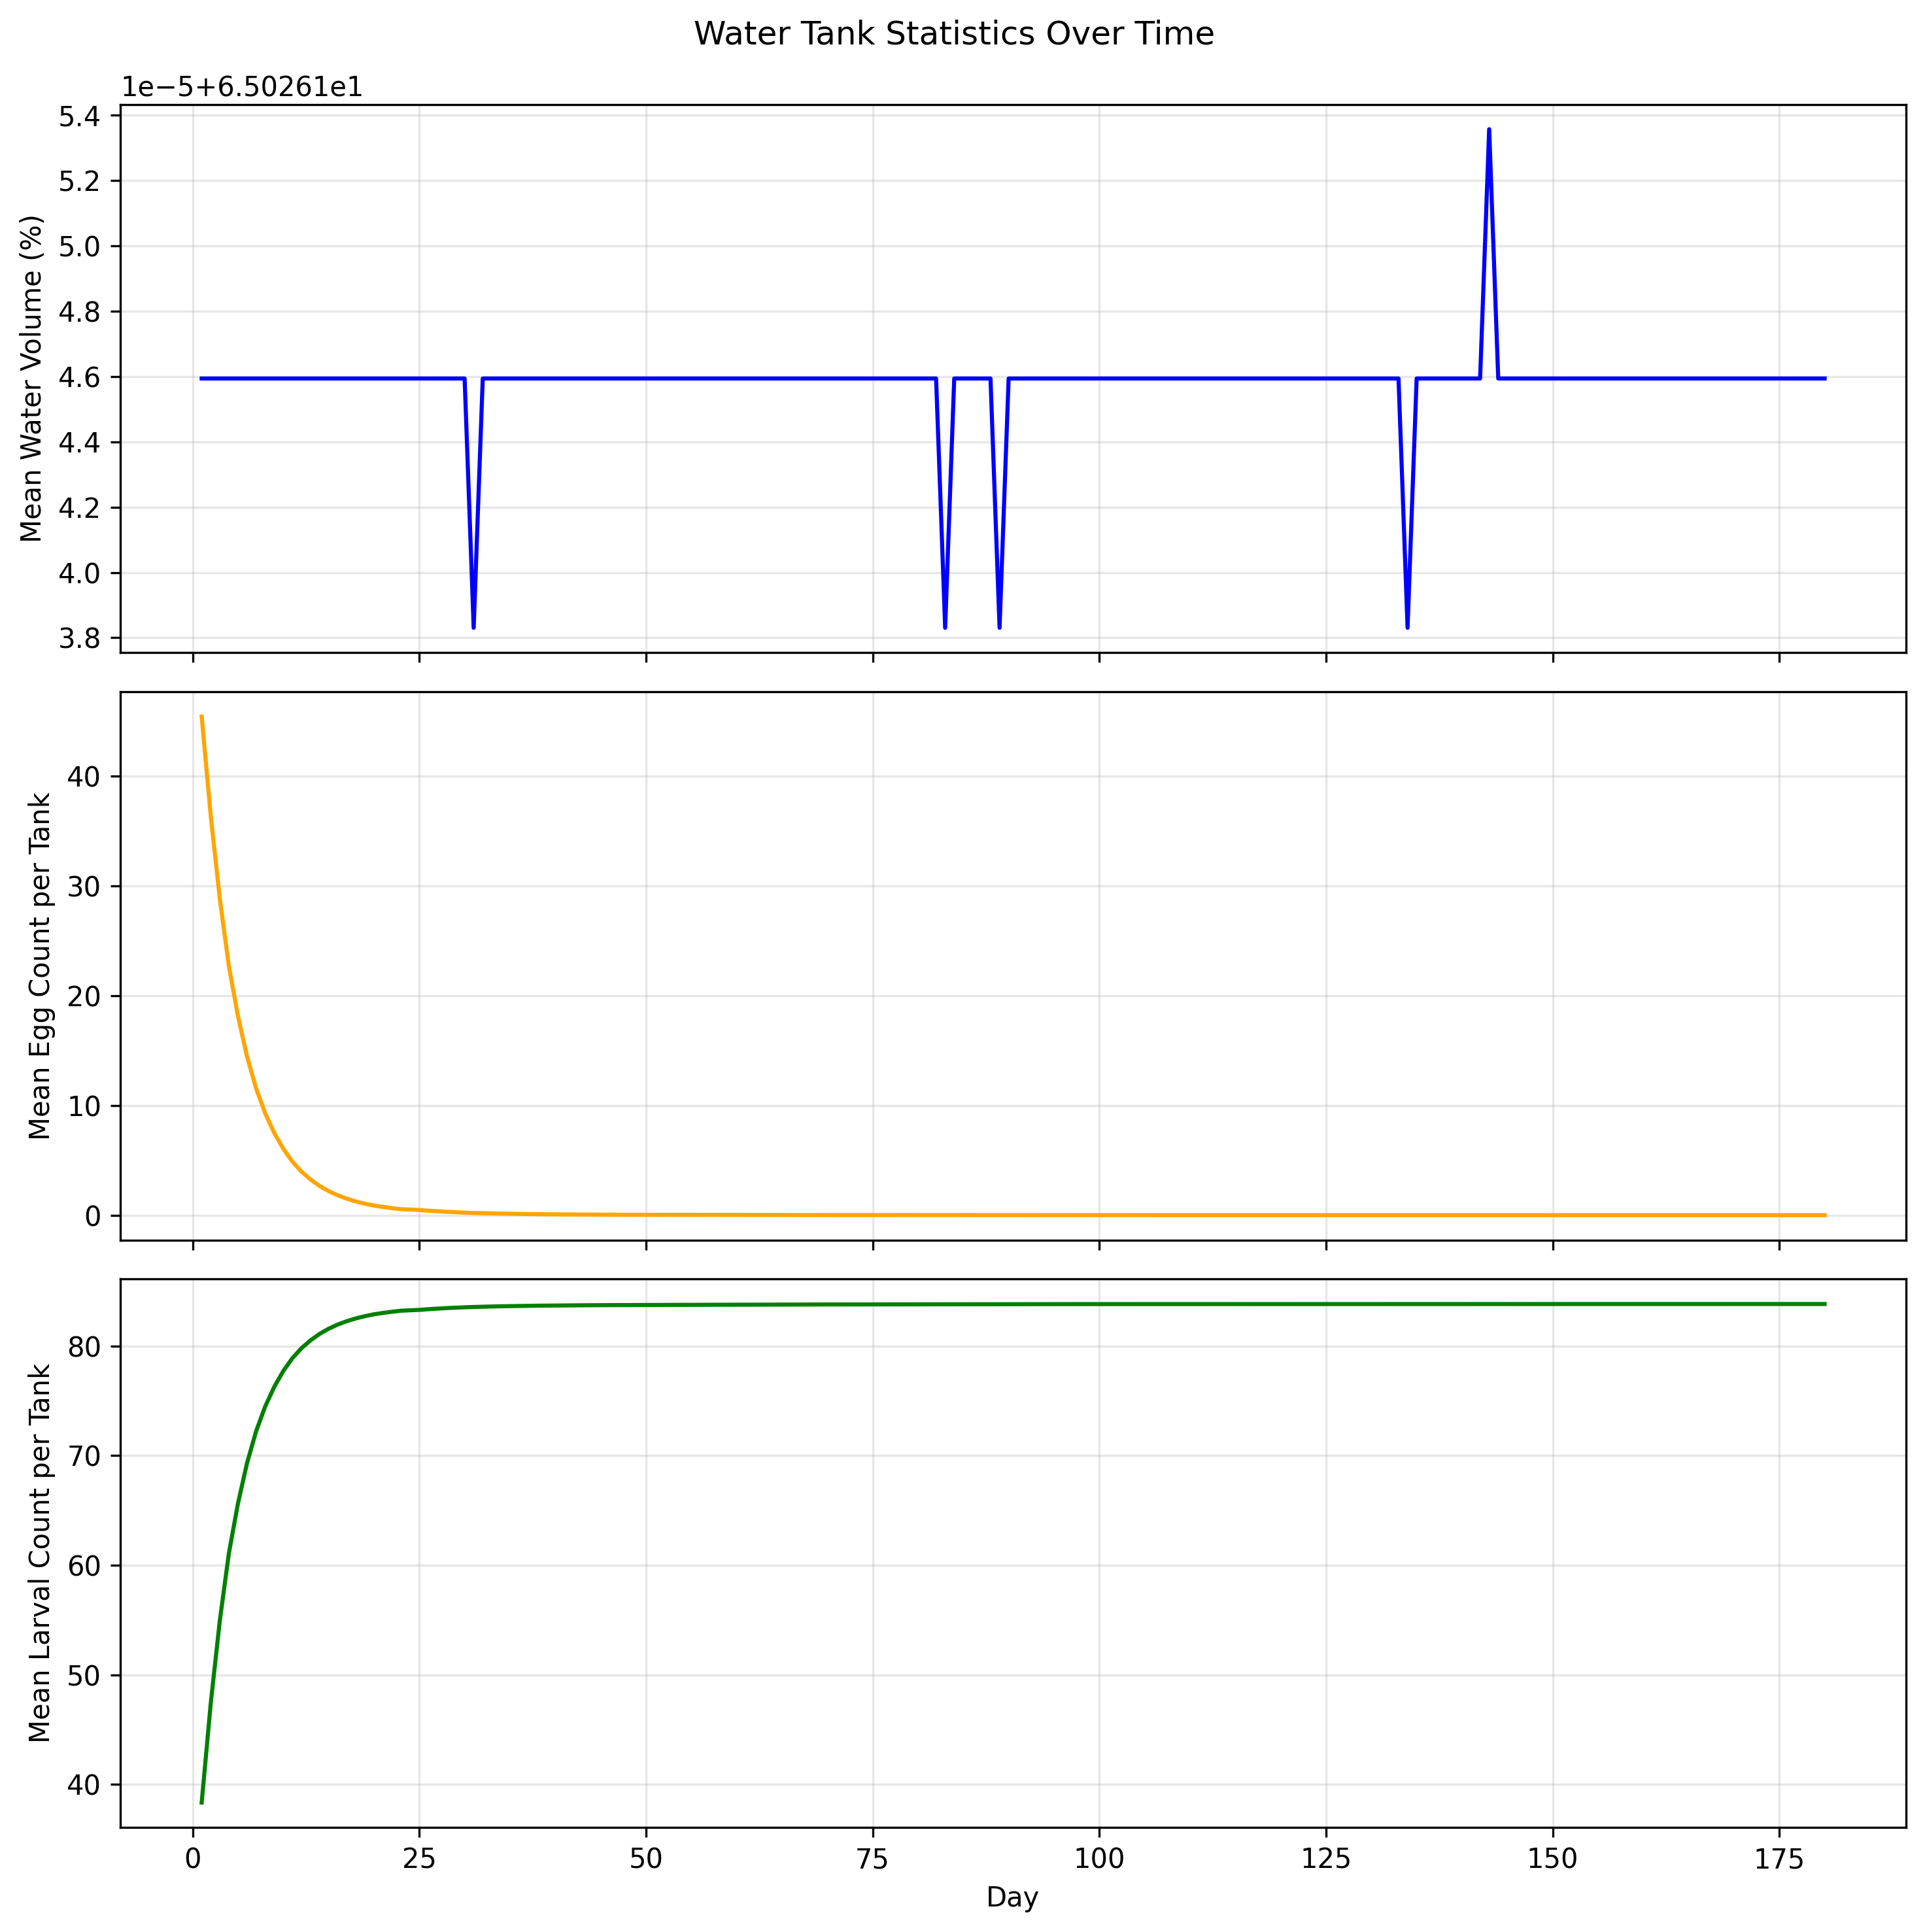
\includegraphics[width=\textwidth]{figs/somali/tank_stats.png}
        \caption{Somali}
    \end{subfigure}
    \hfill
    \begin{subfigure}[b]{0.48\textwidth}
        \centering
        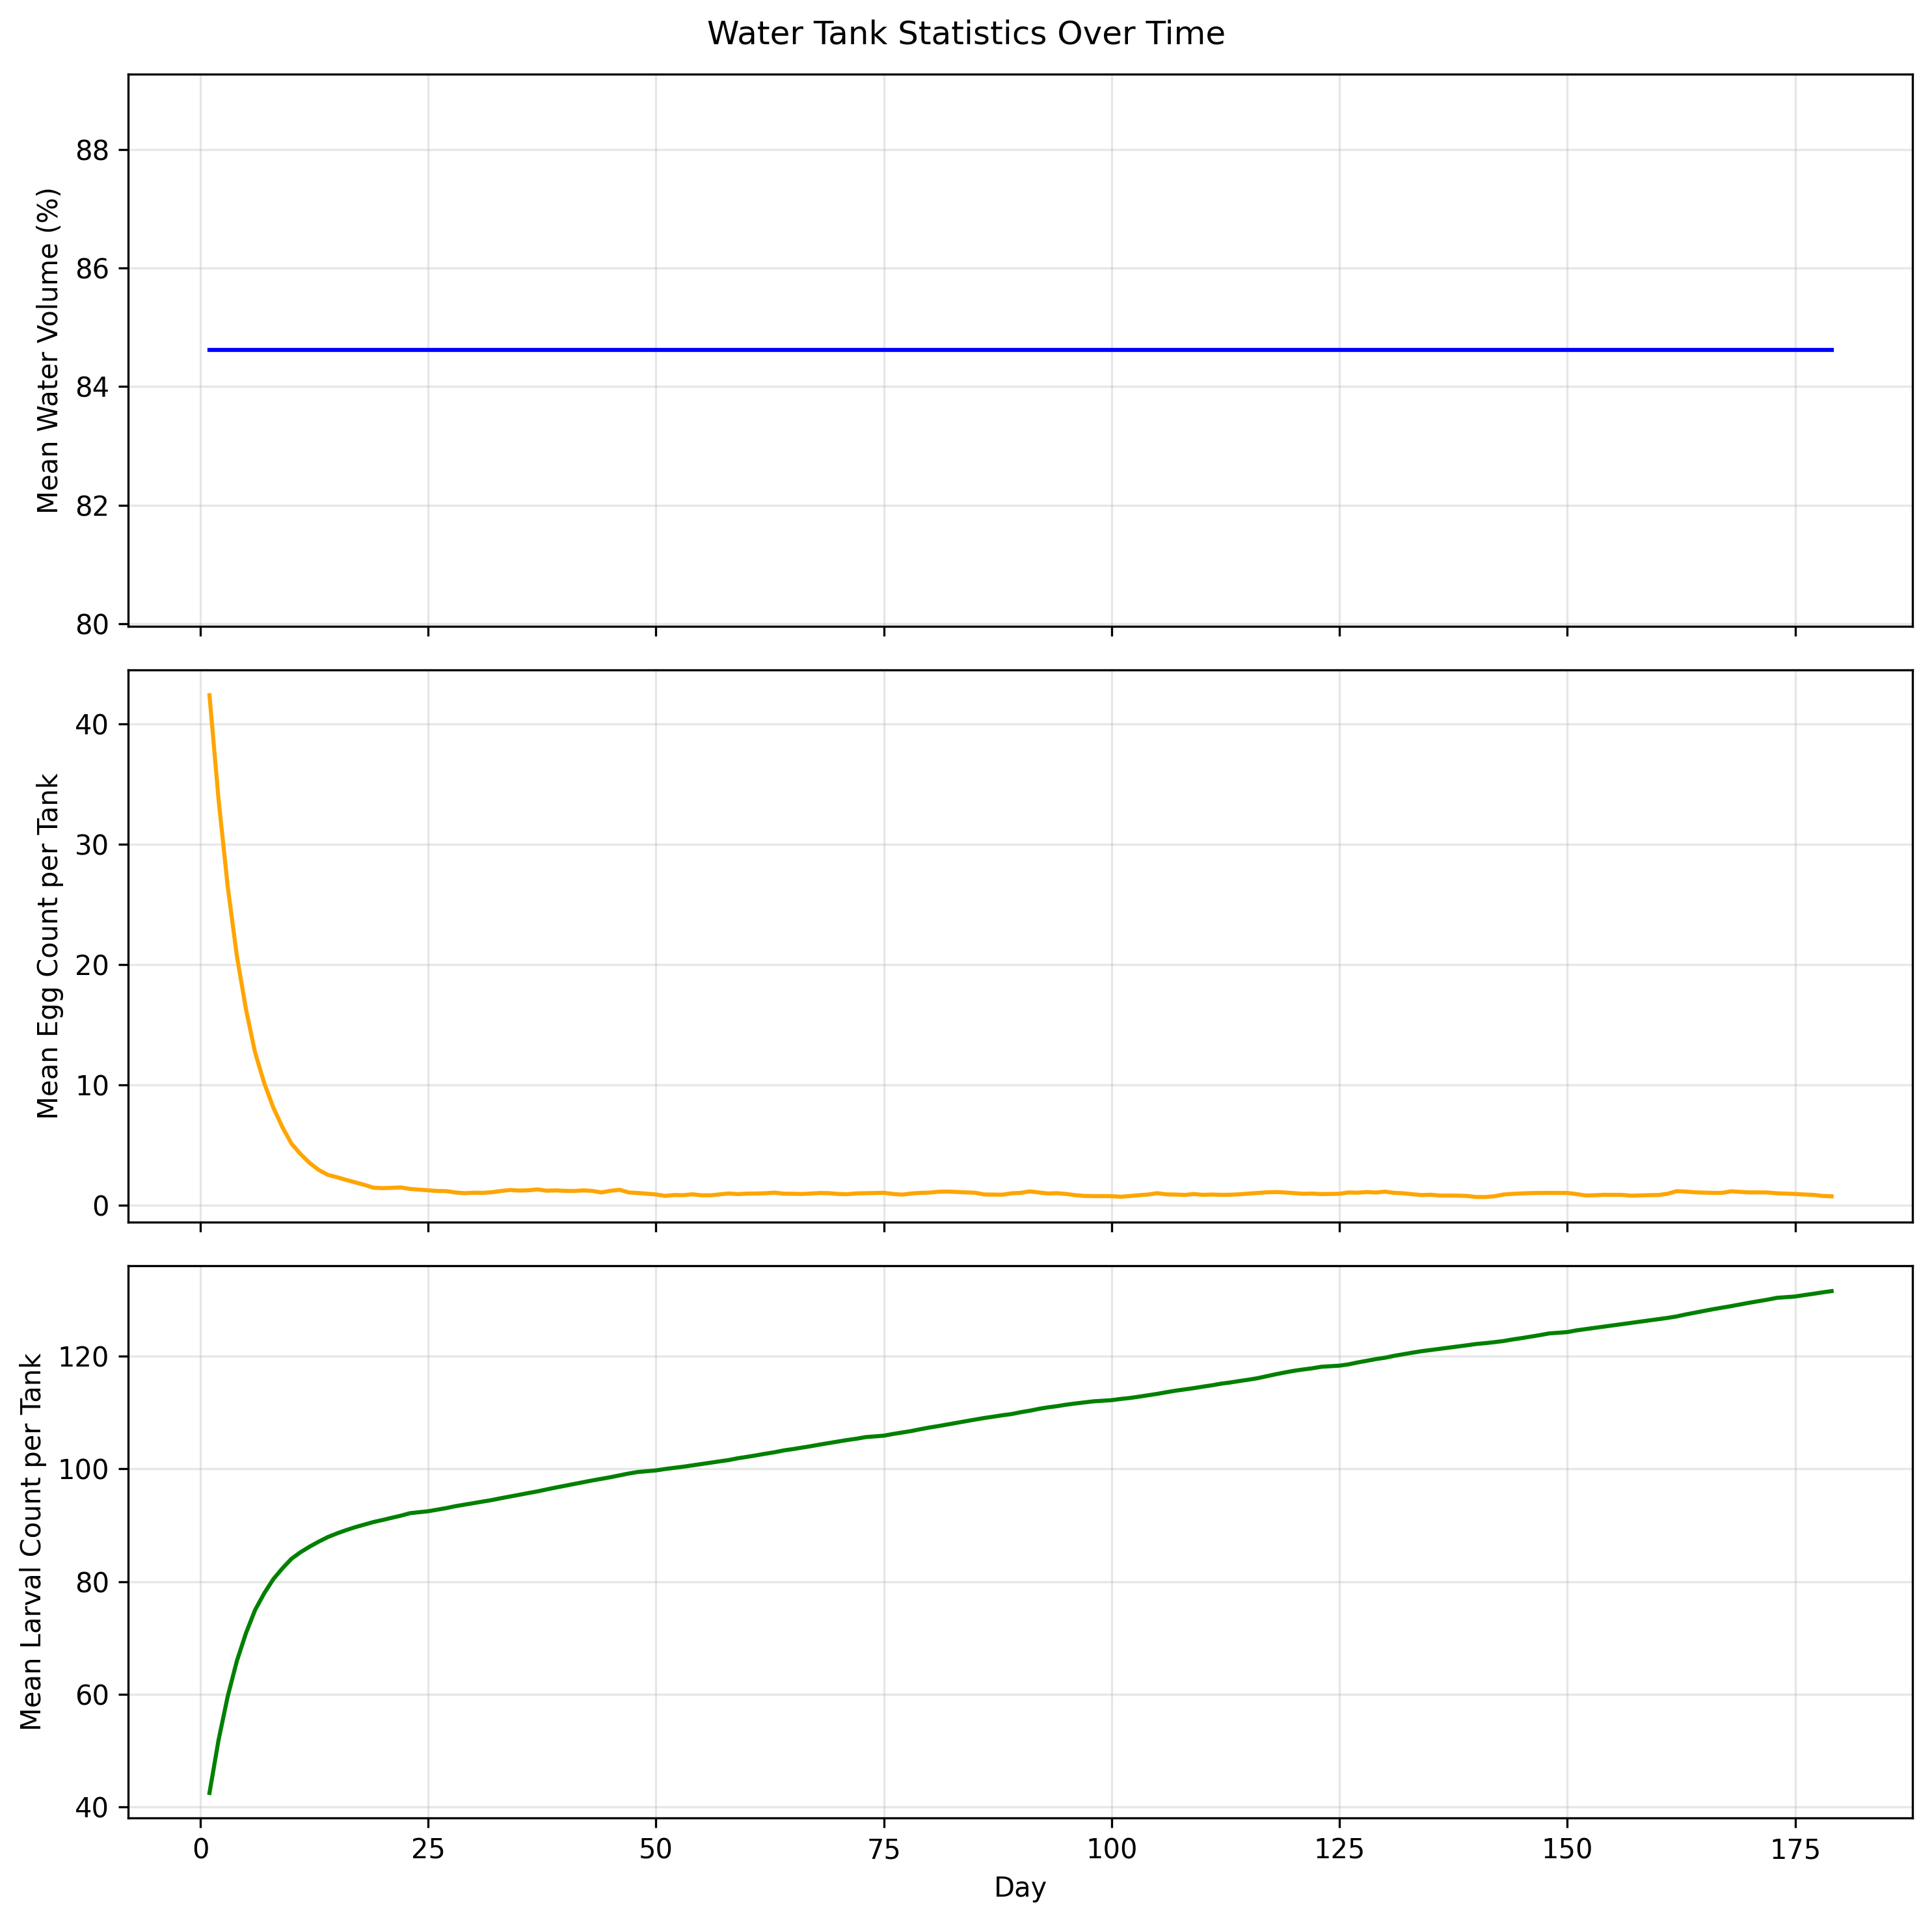
\includegraphics[width=\textwidth]{figs/oromia/tank_stats.png}
        \caption{Oromia}
    \end{subfigure}
    \caption{Water tank statistics: (top) mean water volume; (middle) mean eggs per tank; (bottom) mean larvae per tank.}
    \label{fig:tank_stats}
\end{figure}

\subsection{Environmental Correlation}

Daily average temperatures ranged between \qtyrange{20.7}{23.8}{\celsius} in Oromia and remained almost constant at \qty{26.34}{\celsius} 
in Somali. Precipitation was low and relatively constant in Somali ($\sim \qty{0.058}{\milli\meter\per\day}$), while Oromia experienced 
higher and more variable precipitation (mean \qty{1.35}{\milli\meter\per\day}; Figure~\ref{fig:environment}). The low variability in 
these drivers, especially in Somali, explains the dominance of endogenous population processes over short-term climatic forcing in 
this specific case study.

\begin{figure}[!htb]
    \centering
    \begin{subfigure}[b]{0.48\textwidth}
        \centering
        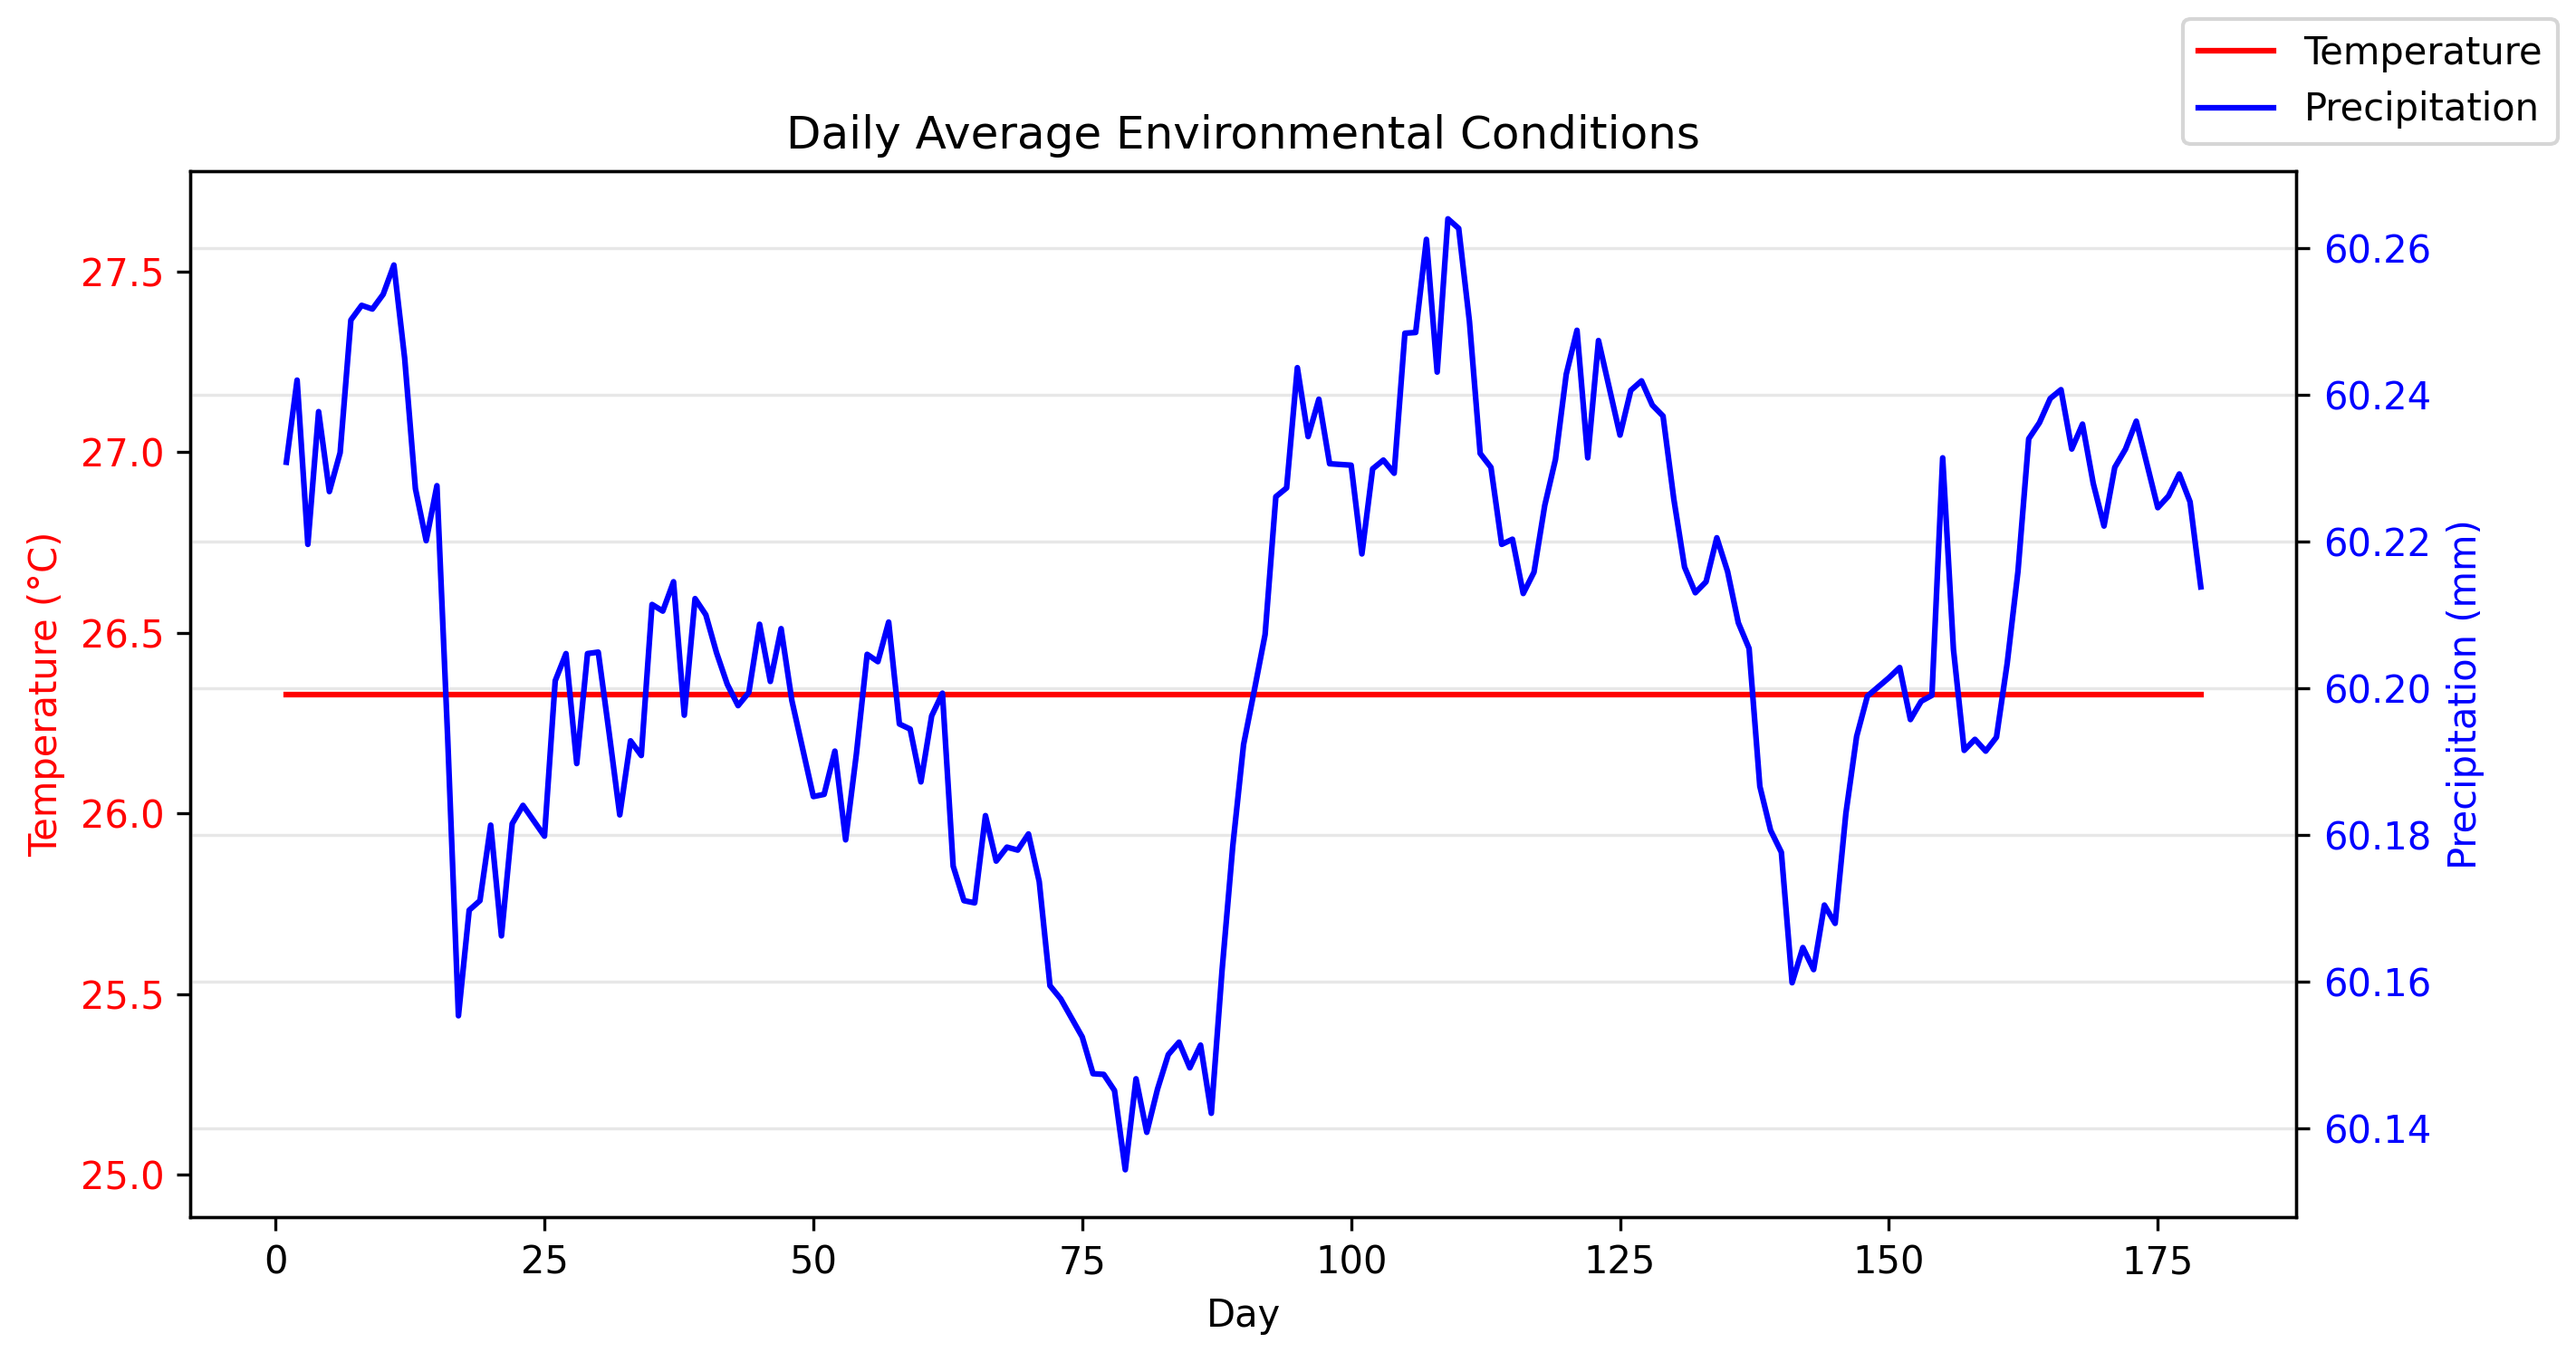
\includegraphics[width=\textwidth]{figs/somali/environment.png}
        \caption{Somali}
    \end{subfigure}
    \hfill
    \begin{subfigure}[b]{0.48\textwidth}
        \centering
        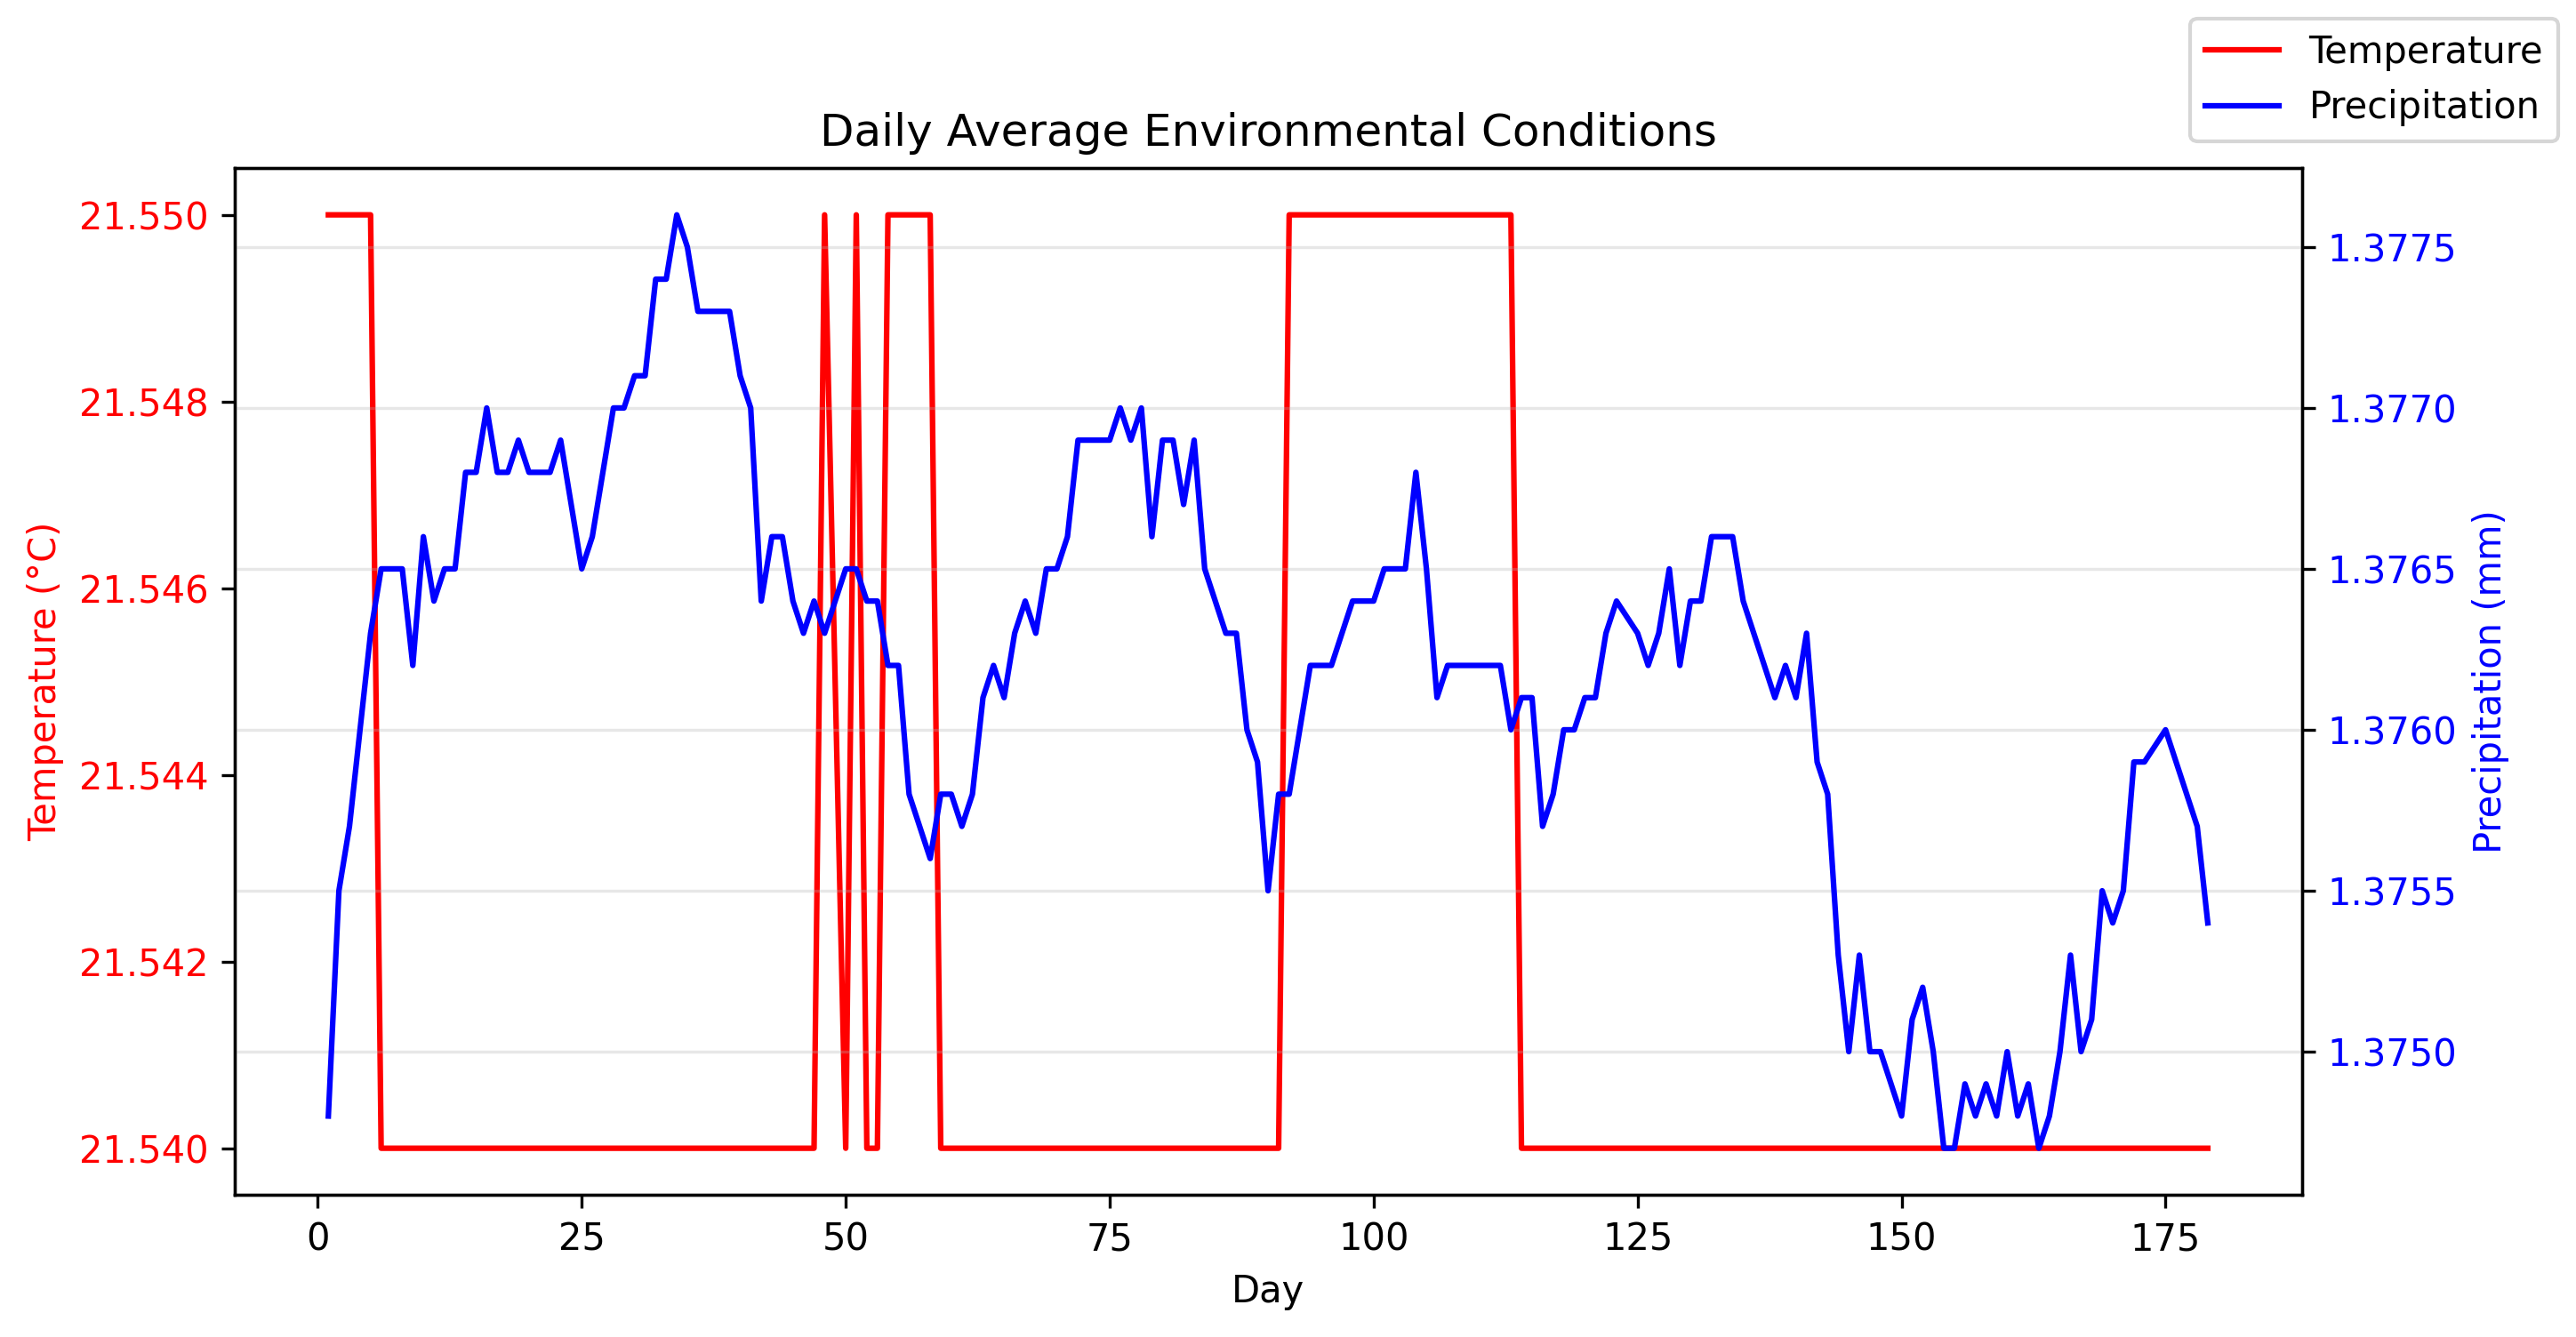
\includegraphics[width=\textwidth]{figs/oromia/environment.png}
        \caption{Oromia}
    \end{subfigure}
    \caption{Daily average environmental conditions (temperature in red, precipitation in blue) throughout the simulation.}
    \label{fig:environment}
\end{figure}

\subsection{Spatial Suitability and Validation}

Spatial suitability maps were generated using Kernel Density Estimation (KDE) with a bandwidth of \qty{0.002}{\degree} 
($\sim \qty{220}{\meter}$). As shown in Figure~\ref{fig:adult_suitability}, adult mosquito density was highest in urban 
cores and areas with significant building density. Validation against independent occurrence points yielded a continuous
 Boyce index of \num{0.504} for Oromia and \num{0.782} for Somali. The proportion of occurrence points falling within the 
 top 20\% of the adult suitability raster was \qty{35.7}{\percent} for Oromia and \qty{36.7}{\percent} for Somali, 
 confirming the model's moderate to good predictive power for invasive vector establishment. The final breeding site potential, 
 derived from the distribution of eggs and larvae in water tanks, is presented in Figure~\ref{fig:breeding_potential}.

\begin{figure}[!htb]
    \centering
    \begin{subfigure}[b]{0.48\textwidth}
        \centering
        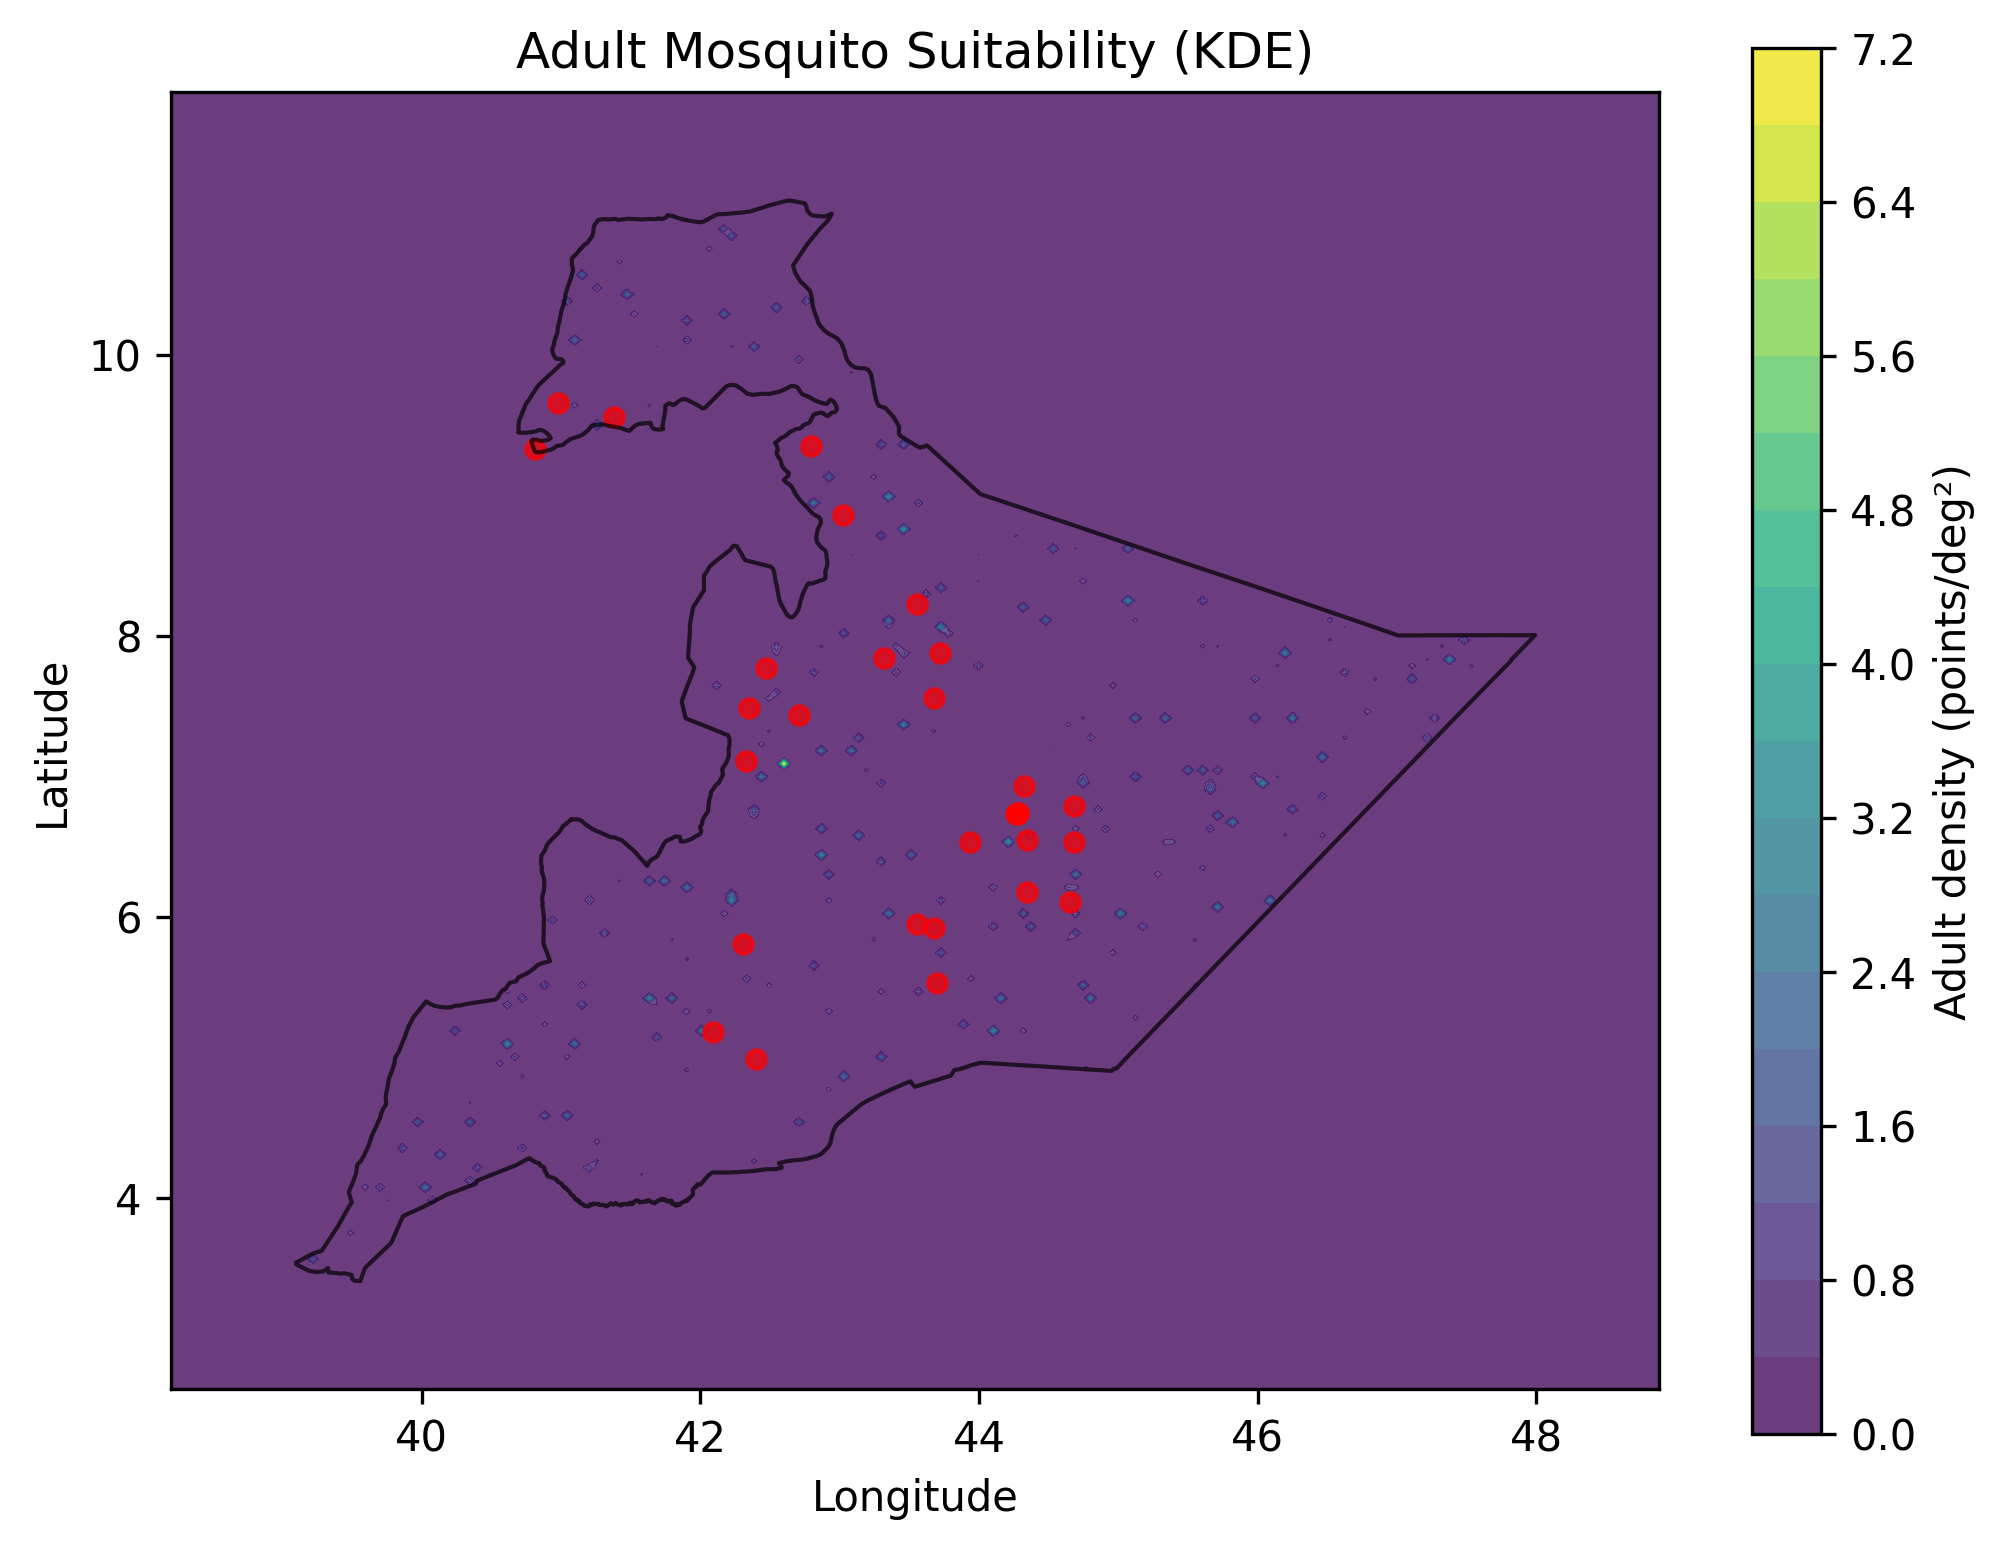
\includegraphics[width=\textwidth]{figs/somali/adult_suitability.png}
        \caption{Somali}
    \end{subfigure}
    \hfill
    \begin{subfigure}[b]{0.48\textwidth}
        \centering
        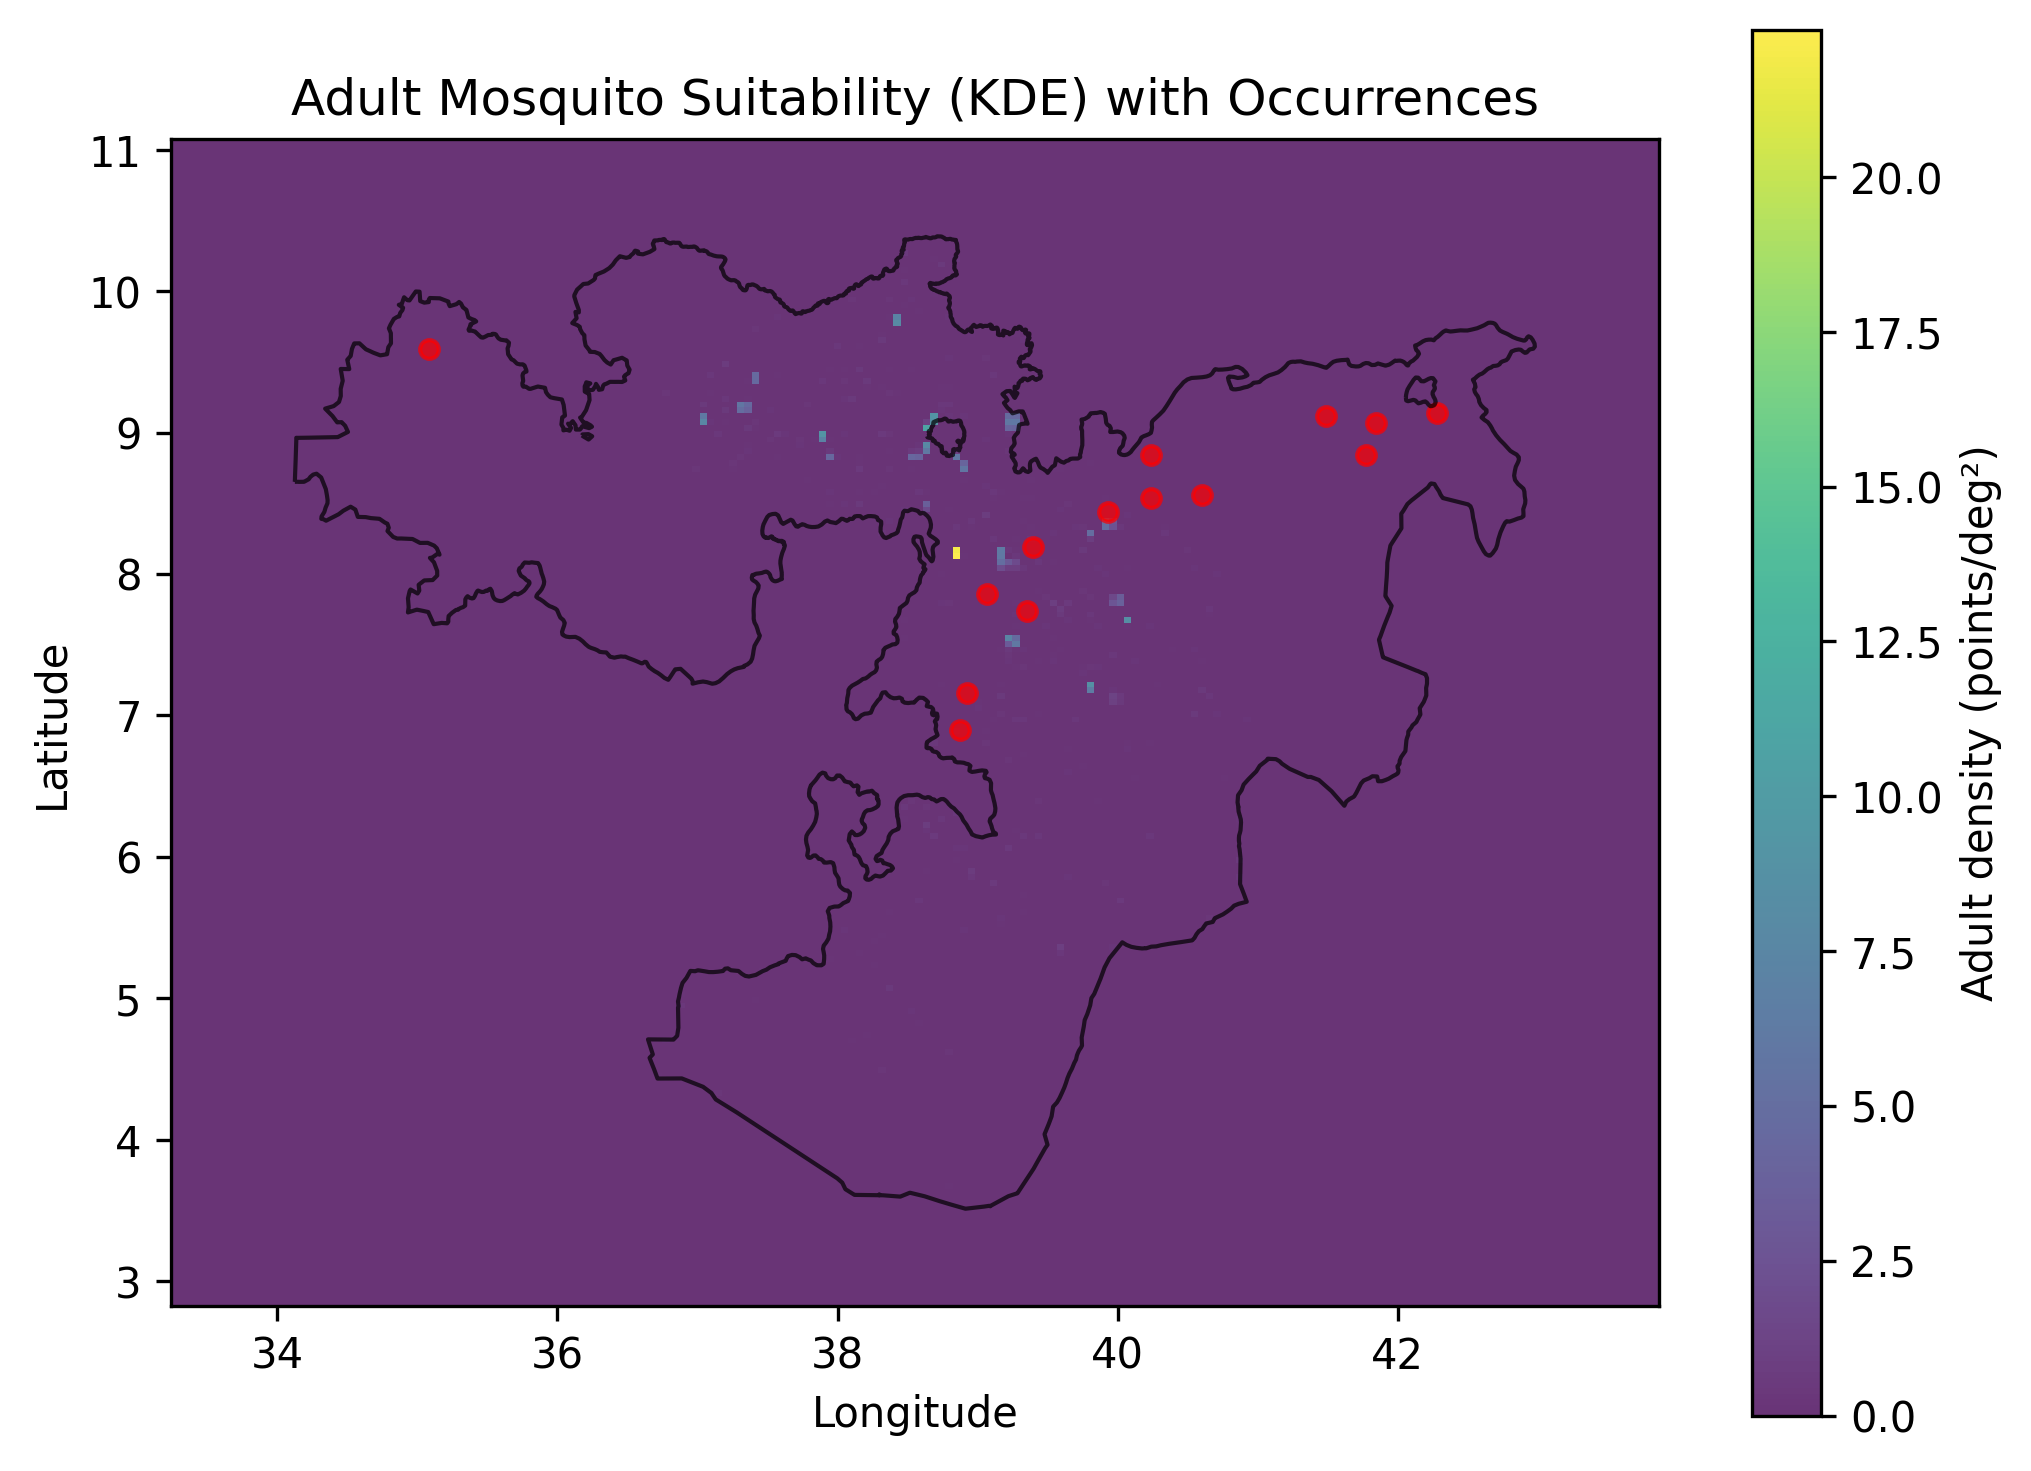
\includegraphics[width=\textwidth]{figs/oromia/adult_suitability.png}
        \caption{Oromia}
    \end{subfigure}
    \caption{Adult mosquito suitability maps (KDE) overlaid with occurrence records (red dots). High density correlates with urban infrastructure.}
    \label{fig:adult_suitability}
\end{figure}

\begin{figure}[!htb]
    \centering
    \begin{subfigure}[b]{0.48\textwidth}
        \centering
        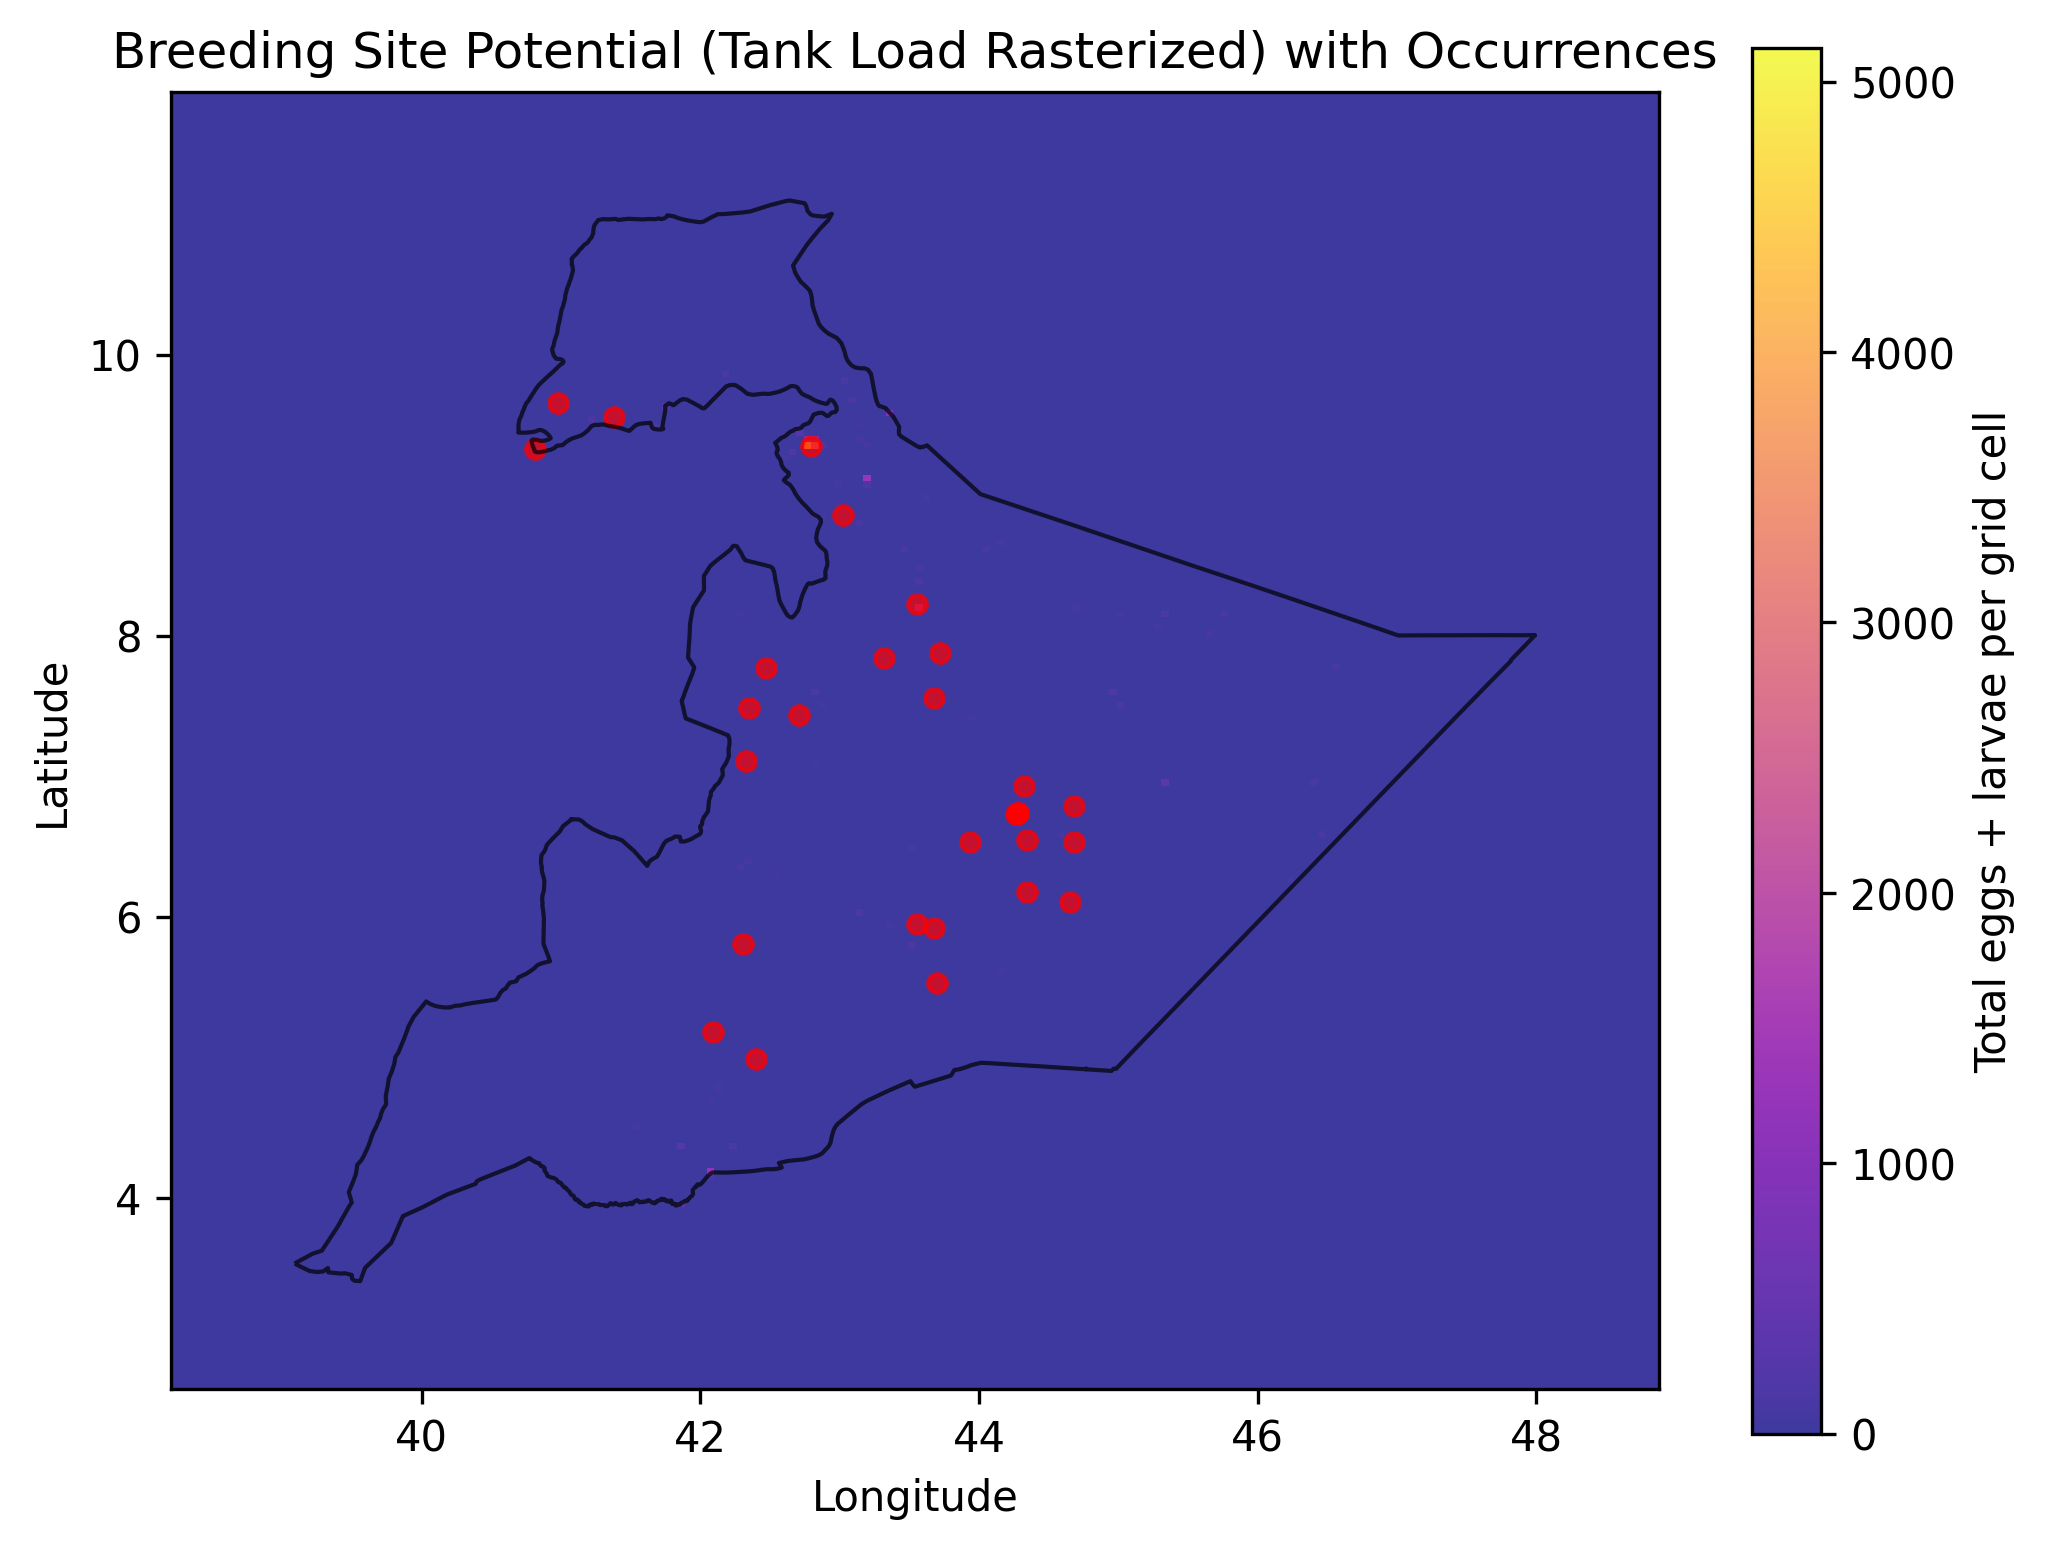
\includegraphics[width=\textwidth]{figs/somali/breeding_site_potential.png}
        \caption{Somali}
    \end{subfigure}
    \hfill
    \begin{subfigure}[b]{0.48\textwidth}
        \centering
        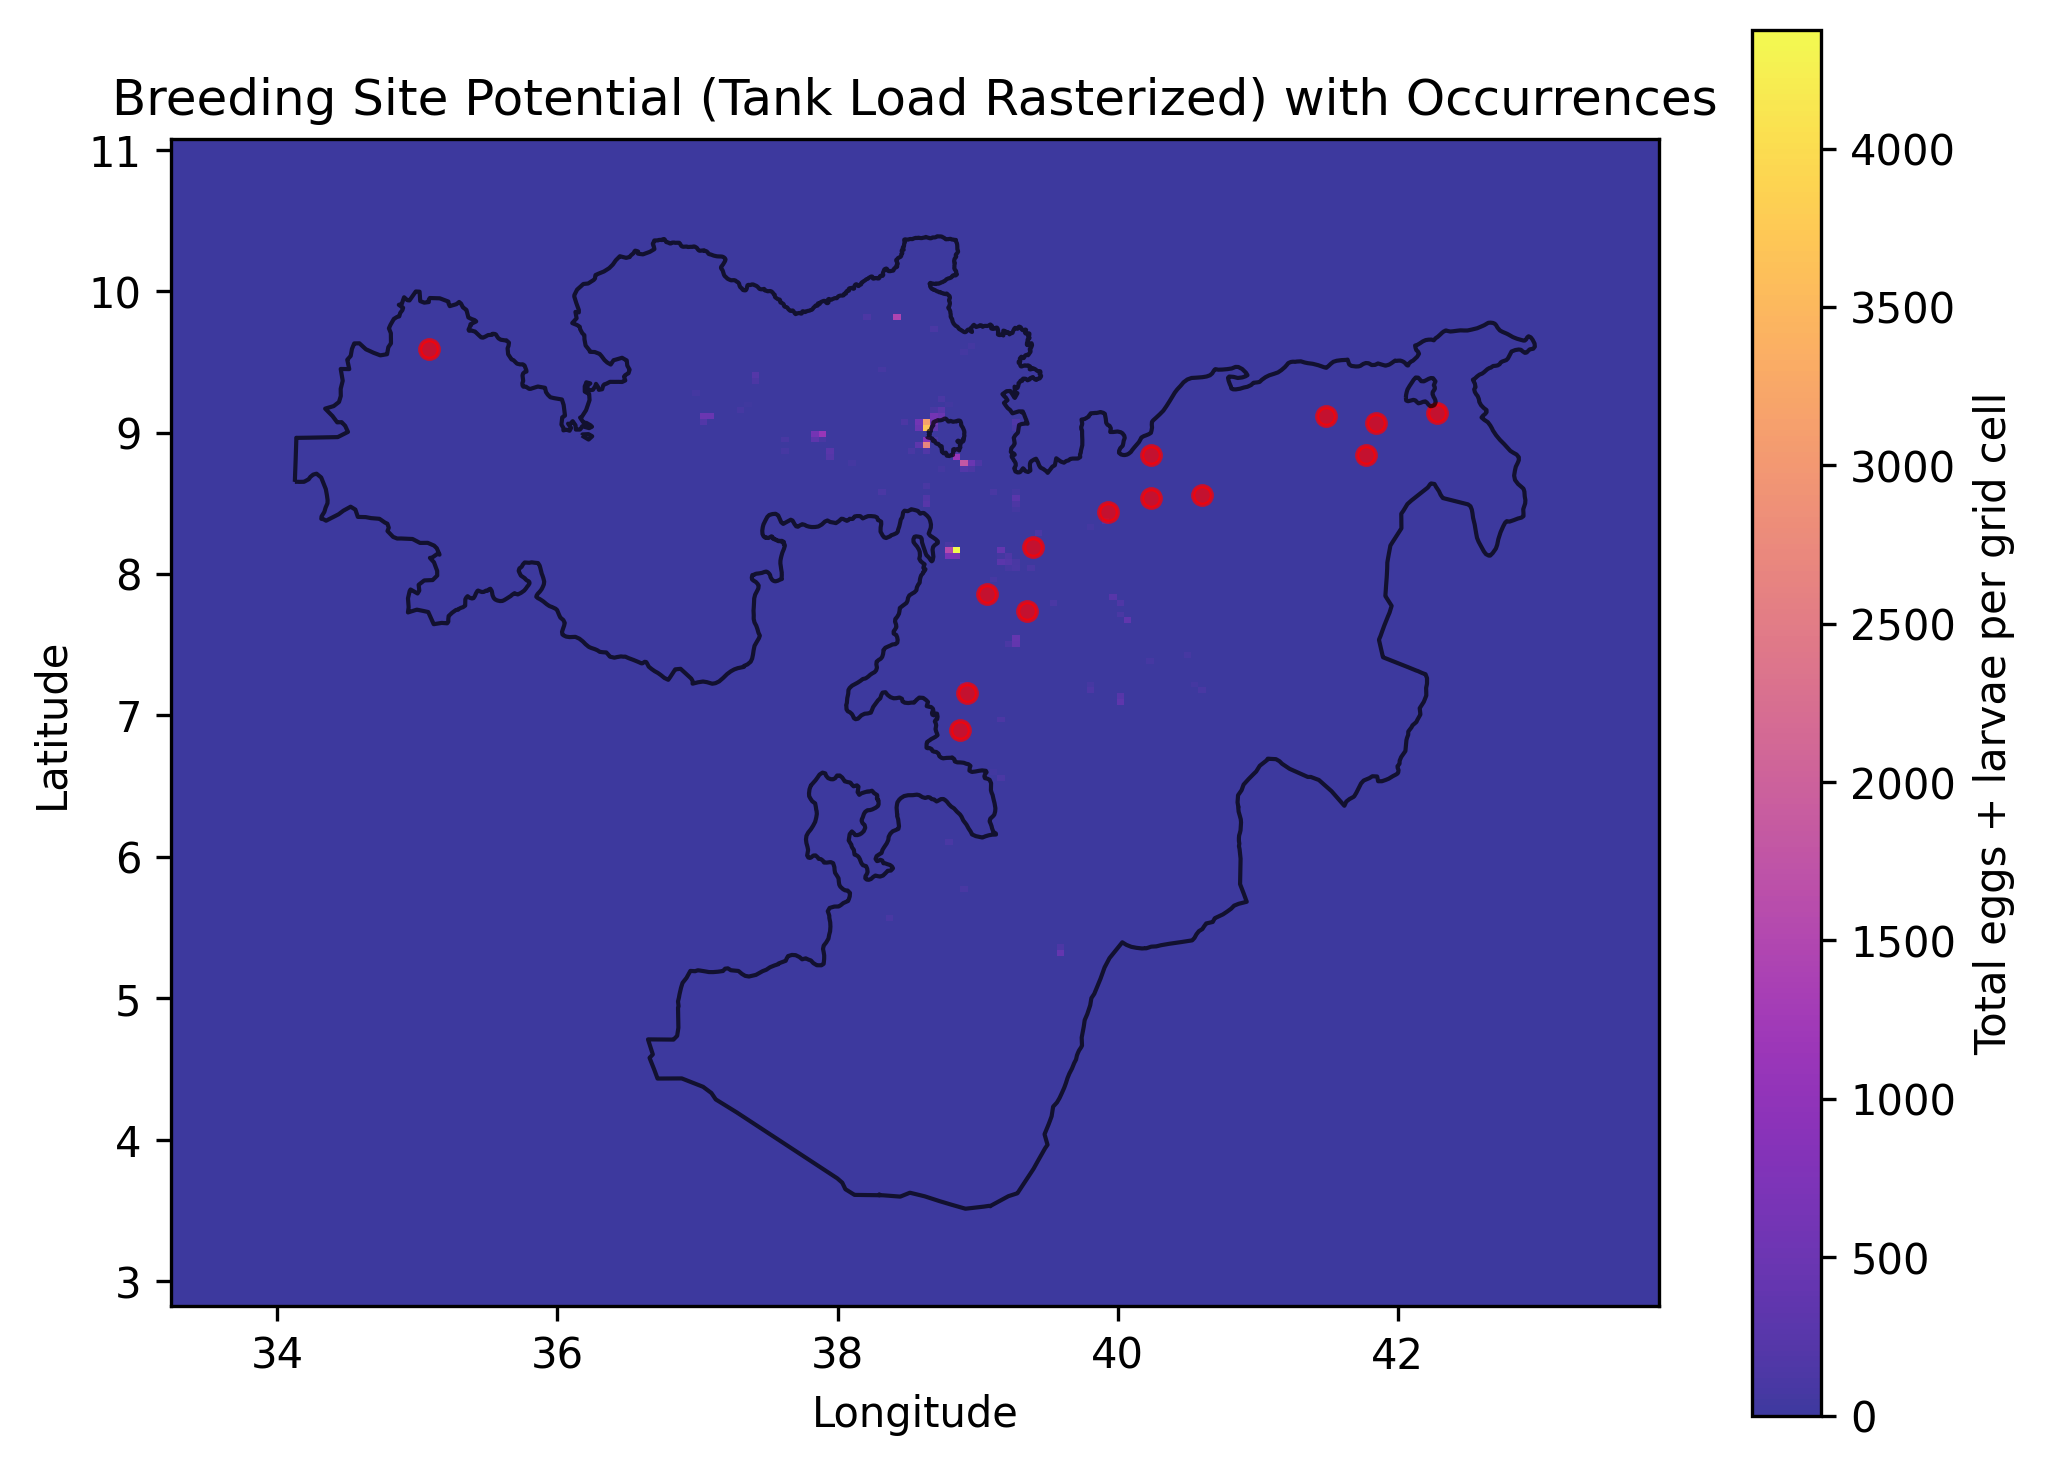
\includegraphics[width=\textwidth]{figs/oromia/breeding_site_potential.png}
        \caption{Oromia}
    \end{subfigure}
    \caption{Breeding site potential rasterized from final egg and larval counts in water tanks, overlaid with occurrence records (red dots).}
    \label{fig:breeding_potential}
\end{figure}

\subsection{Performance Metrics}

Table~\ref{tab:performance} summarises the computational and agent statistics for both study sites. Both simulations completed the 
full 180-day period (\num{17280} ticks) without errors. The Oromia run had a slightly lower total runtime (\qty{2253}{\second} 
vs. \qty{2439}{\second}) and a slightly higher effective frame rate (8.2~FPS) despite having a larger spatial grid 
(\num{60.9} million cells). Memory consumption was significantly higher for the Somali simulation 
(\qty{1305}{\mega\byte} vs. \qty{650}{\mega\byte}) due to the larger number of agents (\num{191092} vs. \num{118614}).

Both runs stayed well below the available memory limit, confirming that a standard laptop can execute the model for 
region-scale simulations. The average tick time remained below \qty{125}{\milli\second}, enabling the simulation of six 
months of vector population dynamics in less than one hour of wall-clock time on consumer hardware.

\begin{table}[!htb]
\centering
\caption{Performance metrics and agent counts for the two simulation runs.}
\label{tab:performance}
\begin{tabular}{l r r}
\toprule
Metric & {Somali} & {Oromia} \\ 
\midrule
Total runtime (s)               & 2439.1 & 2252.9 \\
Average tick time (ms)          & 124.5 & 122.6 \\
Effective FPS                   & 8.0 & 8.2 \\
Peak memory usage (MB)          & 1305 & 650 \\
Memory utilisation (\% of max)  & 69.5 & 33.3 \\
Total agents (end)              & 191092 & 118614 \\
\quad Mosquitoes                & 191050 & 118140 \\
\quad Water tanks               & 42 & 474 \\
Rule evaluations                & 6716 & 6603 \\
Actions executed                & 18512932 & 19650028 \\
Spatial registry --- inserts    & 224614 & 194738 \\
Spatial registry --- updates    & 151 & 138 \\
Max agents per spatial cell     & 513 & 319 \\ 
\bottomrule
\end{tabular}
\end{table}


\section{Discussion}
\label{sec:discussion}
\par
The simulation results demonstrate that the agent-based model successfully reproduces population dynamics for 
\textit{Anopheles stephensi} across two distinct Ethiopian ecological settings. In the Oromia \textit{woredas}, 
the population maintained a near-equilibrium state with an average predicted $\lambda_{\max}$ of \num{1.077}, 
whereas in Somali, the model predicted a more robust growth potential ($\lambda_{\max} = 1.135$). These findings 
align with field reports that identify Somali as a primary hotspot for the species' establishment in urban 
Ethiopia \citep{2021.MB.AUO}. The theoretical stage durations -- \qty{15.7}{\day} for larvae and \qty{4.8}{\day} 
for pupae in Oromia (\qty{21.5}{\celsius}) and \qty{11.4}{\day} and \qty{4.3}{\day}, respectively, in the warmer Somali 
region (\qty{26.3}{\celsius}) -- fall within the ranges reported in laboratory studies~\citep{2023.JJ.BBA}, supporting 
the validity of our temperature-dependent parameterisation.
\par
A key finding is the site-specific response to environmental drivers. In Oromia, adult abundance showed a weak positive 
correlation with temperature ($r = 0.119$, $p = 0.12$) and a stronger positive correlation with precipitation 
($r = 0.618$, $p = \num{1.6e-19}$), suggesting that precipitation may enhance larval habitat availability and adult 
survivorship. In Somali, where temperature remained almost constant, a moderate negative correlation was observed between 
adult counts and precipitation ($r = -0.477$, $p = \num{3.8e-11}$), potentially reflecting a ``wash-out'' effect or a shift 
in habitat availability during high-rainfall events, a phenomenon documented for urban container-breeding mosquitoes 
elsewhere \citep{2016.ST.OTI}. These contrasting responses underscore the importance of local hydro-climatic contexts 
when modelling \textit{An.~stephensi} stability.
\par
The spatial suitability maps generated via KDE correctly highlighted urban cores and high-building-density areas as the most 
suitable habitats. Validation against independent occurrence points yielded a Continuous Boyce Index (CBI) of \num{0.504} 
for Oromia and \num{0.782} for Somali, indicating moderate to high predictive performance for both regions. The proportion 
of occurrence points falling within the top \qty{20}{\percent} of predicted suitability areas was \qty{35.7}{\percent} for 
Oromia and \qty{36.7}{\percent} for Somali, confirming that the model effectively captures high-risk zones across different 
spatial settings.
\par
The performance analysis (Table~\ref{tab:performance}) demonstrates that the simulation framework is computationally efficient 
and can run on modest hardware. Both six-month simulations completed in less than \qty{2450}{\second} (approximately \qty{40}{\minute}) 
on a standard laptop, with average tick times below \qty{125}{\milli\second}. Peak memory usage remained \qty{1317}{\mega\byte} 
for the larger Somali simulation (\num{191}k agents) and \qty{650}{\mega\byte} for the Oromia simulation (\num{119}k agents), 
well under the \qty{2}{\giga\byte} heap limit. Notably, the Oromia simulation handled a very sparse spatial grid of \num{60.9} 
million cells (due to the larger study area) with only \num{474} water tanks, while the Somali simulation used a grid of \num{68.5} 
million cells with \num{42} tanks. The lazy spatial registry kept performance acceptable despite the vast number of empty cells, with 
rule evaluations and actions executed remaining within practical limits. These characteristics are critical for deployment in sub-Saharan 
African public health institutions, where access to high-performance computing clusters is often limited.
\par
This opens the door for routine use by national malaria control programs and regional health observatories, enabling them to run 
scenario analyses, evaluate intervention strategies, and generate risk maps using only standard office computers. Future work will 
focus on reducing the memory footprint further and providing user-friendly interfaces to lower the technical barrier for public health 
officers in endemic areas.
\par
Several limitations should be acknowledged. The current movement rules utilise a random walk with a fixed step size, which may not 
fully capture complex host-seeking behaviours toward specific resource gradients. Furthermore, the model assumes human population density 
is the sole proxy for blood-meal availability. Given that \textit{An. stephensi} exhibits plastic feeding behaviour, including zoophily, 
a multi-host formulation might improve fecundity estimates in peri-urban areas. Despite these limitations, we believe the framework 
provides a valuable tool for designing targeted vector control interventions. The YAML-driven parameterisation allows for rapid 
adaptation to other regions or species. Future research should extend these simulations to multi-year runs to evaluate the impact 
of long-term climate variability and the effectiveness of larval source management, such as the systematic covering of water tanks, 
on population suppression.


\section{Conclusion}
\label{sec:conclusion}
\par
This study presented an agent--based modelling framework for simulating the population dynamics of mosquitoes in low--resource settings, 
with a case study on \textit{Anopheles stephensi} in two Ethiopian regions (Somali and Oromia). The model successfully integrated 
temperature--dependent life--history traits with spatially explicit environmental data and a stage--structured Metzler matrix. 
The framework was applied to Somali and Oromia using six--month simulations driven by ERA5--Land data. 
\par
The results demonstrated that the simulated populations reached near--equilibrium or slowly growing states consistent with field 
observations of established vectors. In Oromia, the average predicted $\lambda_{\max}$ was \num{1.077}, and the adult population 
stabilised at approximately \num{85000} individuals. In Somali, a higher growth potential ($\lambda_{\max} = 1.135$) was observed, 
with adult numbers starting at \num{131000} and continuing a slow increase. The model identified significant regional differences 
in climatic sensitivities: Oromia showed positive correlations with both temperature and precipitation, while Somali (with nearly 
constant temperature) exhibited a moderate negative correlation with precipitation. Validation against independent occurrence data 
yielded Continuous Boyce Indices of \num{0.504} for Oromia and \num{0.782} for Somali, with \qty{35.7}{\percent} and \qty{36.7}
{\percent} of occurrence points falling within the top \qty{20}{\percent} of suitability, respectively. These results confirm 
the model's ability to identify urban hotspots even in data--poor environments.
\par
Computational performance was adequate for routine use: both six--month simulations completed in less than \qty{2450}{\second} on 
standard laptop hardware, with average tick times below \qty{125}{\milli\second} and peak memory usage under \qty{1.4}{\giga\byte}. 
While limitations regarding adult dispersal and host--seeking behaviour remain, the framework provides a generic, reusable, and 
easily parameterisable tool for public health decision--making. By linking life--cycle biology with spatial infrastructure data, 
the model could support evidence--based planning of larval source management and urban malaria control programmes in recently 
invaded territories.


\section*{Data availability}
\label{sec:data_availability}
The code of the simulator and the data used for the case study are all available in a github directory:
\url{https://github.com/Vansnoden/monadvsim}.


\section*{Acknowledgments}
\par
This research was supported by the International Center of Insect Physiology and Ecology (ICIPE), 
the University of KwaZulu-Natal, and the International Institute of Tropical Agriculture (IITA). 
We acknowledge the providers of the open data used in this study, including GBIF, the Copernicus 
Climate Change Service (ERA5-Land), the Malaria Atlas Project, and the Vector Atlas consortium. 
We particularly thank the data contributors and curators who make their work publicly available, 
enabling research of this nature.


\bibliographystyle{apalike}
\bibliography{bibliography.bib}

\end{document}
